
\title{Case-Enabled Reasoning Engine with Bayesian Representations for Unified Modeling (CEREBRUM)}
\author{Daniel Ari Friedman}
\date{Version 1.0 (2025-04-07)}

\begin{document}
\maketitle


\renewcommand{\contentsname}{Contents}
{
\setcounter{tocdepth}{2}
\tableofcontents
}

% Main body content before the appendices

% Main document content
\hypertarget{cerebrum-case-enabled-reasoning-engine-with-bayesian-representations-for-unified-modeling}{%
\chapter{CEREBRUM: Case-Enabled Reasoning Engine with Bayesian
Representations for Unified
Modeling}\label{cerebrum-case-enabled-reasoning-engine-with-bayesian-representations-for-unified-modeling}}

\textbf{Daniel Ari Friedman}

\emph{Active Inference Institute}

ORCID: 0000-0001-6232-9096

Email: daniel@activeinference.institute

Version 1.0 (2025-04-07) \textasciitilde{} CC BY-NC-ND 4.0

\hypertarget{abstract}{%
\section{Abstract}\label{abstract}}

This paper introduces Case-Enabled Reasoning Engine with Bayesian
Representations for Unified Modeling (CEREBRUM). CEREBRUM is a synthetic
intelligence framework that integrates linguistic case systems with
cognitive scientific principles to describe, design, and deploy
generative models in an expressive fashion. By treating models as
case-bearing entities that can play multiple contextual roles (e.g.~like
declinable nouns), CEREBRUM establishes a formal linguistic-type
calculus for cognitive model use, relationships, and transformations.
The CEREBRUM framework uses structures from category theory and modeling
techniques related to the Free Energy Principle, in describing and
utilizing models across contexts. CEREBRUM addresses the growing
complexity in computational and cognitive modeling systems
(e.g.~generative, decentralized, agentic intelligences), by providing
structured representations of model ecosystems that align with lexical
ergonomics, scientific principles, and operational processes.

\hypertarget{overview}{%
\section{Overview}\label{overview}}

CEREBRUM implements a comprehensive approach to cognitive systems
modeling by applying linguistic case systems to model management. This
framework treats cognitive models as entities that can exist in
different ``cases'', as in a morphologically rich language, based on
their functional role within an intelligence production workflow. This
enables more structured representation of model relationships and
transformations.

The code to generate this paper, and further open source development
from this 1.0 milestone release, is available at
https://github.com/ActiveInferenceInstitute/CEREBRUM .

\hypertarget{background}{%
\section{Background}\label{background}}

\hypertarget{cognitive-systems-modeling}{%
\subsection{Cognitive Systems
Modeling}\label{cognitive-systems-modeling}}

Cognitive systems modeling approaches cognition as a complex adaptive
system, where cognitive processes emerge from the dynamic interaction of
multiple components across different scales. This perspective draws from
ecological psychology's emphasis on organism-environment coupling, where
cognitive processes are fundamentally situated in and shaped by their
environmental context. The 4E cognition framework (embodied, embedded,
enacted, and extended) provides a theoretical foundation for
understanding how cognitive systems extend beyond individual agents to
include environmental structures and social interactions. In this view,
cognitive models are not merely internal representations but active
participants in a broader cognitive ecosystem, where they adapt and
evolve through interaction with other models and environmental
constraints. This systems-level perspective is particularly relevant for
intelligence production, where multiple analytical models must
coordinate their activities while maintaining sensitivity to changing
operational contexts and requirements. The complex adaptive systems
approach emphasizes self-organization, emergence, and adaptation,
viewing cognitive processes as distributed across multiple interacting
components that collectively produce intelligent behavior through their
coordinated activity (including language use).

\hypertarget{active-inference}{%
\subsection{Active Inference}\label{active-inference}}

Active Inference is a first-principles account of perception, learning,
and decision-making based on the Free Energy Principle. In this
framework, cognitive systems minimize variational free energy ---
bounded surprise, reflecting the difference between an organism's
internal model and its environment --- through perception (updating
internal models) and action (changing action and ultimately sensory
inputs). The Active Inference framework formalizes uncertainty in terms
of entropy and precision weighting, enabling dynamic adaptive processes.
While many model architectures are possible, hierarchical message
passing is a common implementation that implements predictions as
top-down flows and prediction errors as bottom-up flows, creating a
bidirectional inference system that iteratively minimizes surprise
across model levels. Active Inference treats all cognitive operations as
Bayesian model update, providing a unifying mathematical formalism for
predictive cognition.

\hypertarget{linguistic-case-systems}{%
\subsection{Linguistic Case Systems}\label{linguistic-case-systems}}

Linguistic case systems represent grammatical relationships between
words through morphological marking. Case systems operate as
morphosyntactic interfaces between semantics and syntax, encoding
contextualized relationship types rather than just sequential ordering.
This inherent relationality makes case systems powerful abstractions for
modeling complex dependencies and transformations between conceptual
entities. Cases under consideration here include nominative (subject),
accusative (object), dative (recipient), genitive (possessor),
instrumental (tool), locative (location), and ablative (origin), all
serving different functional roles within sentence structures. Languages
implement these differently: nominative-accusative systems distinguish
subjects from objects, while ergative-absolutive systems group
intransitive subjects with direct objects. While English has largely
lost its morphological case system, the underlying case relationships
still exist and are expressed through word order and prepositions. For
example, in ``The cat chased the mouse,'' the nominative case is marked
by position (subject before verb) rather than morphology, while in ``I
gave him the book,'' the dative case is marked by the preposition ``to''
(implied) and word order. This demonstrates that (the
semantics/semiosis/pragmatics of) case relationships are fundamental to
language structure, even when not overtly marked morphologically
(e.g.~expressed in writing or spoken language).

\hypertarget{intelligence-case-management-systems}{%
\subsection{Intelligence Case Management
Systems}\label{intelligence-case-management-systems}}

Intelligence case management systems organize investigative workflows
and analytical processes in operational contexts. These systems
structure information collection, analysis, evaluation, and
dissemination while tracking provenance and relationships between
intelligence products. Modern implementations increasingly must manage
complex model ecosystems where analytical tools, data sources, and
products interact within organizational workflows. However, current
frameworks lack formal mathematical foundations for representing model
relationships, leading to ad hoc integration approaches that become
unwieldy at scale. As artificial intelligence components proliferate in
these systems, a more rigorous basis for model interaction becomes
essential for maintaining operational coherence and analytical
integrity.

\hypertarget{towards-languages-for-generative-modeling}{%
\section{Towards Languages for Generative
Modeling}\label{towards-languages-for-generative-modeling}}

The Active Inference community has extensively explored numerous
adjectival modifications of the base framework, including Deep,
Affective, Branching-Time, Quantum, Mortal, Structured Inference, among
others. Each adjectival-prefixed variant emphasizes specific
architectural aspects or extensions of the core formalism. Building on
this, CEREBRUM focuses on a wider range of linguistic formalism (e.g.~in
this paper, declensional semantics) rather than adjectival
modifications.

In this first CEREBRUM paper, there is an emphasis on the declensional
aspects of generative models as noun-like entities, separate from
adjectival qualification. This approach aligns with category theoretic
approaches to linguistics, where morphisms between objects formalize
grammatical relationships and transformations. By applying formal case
grammar to generative models, CEREBRUM extends and transposes structured
modeling approaches to ecosystems of shared intelligence, while
preserving the underlying (partitioned, flexible, variational,
composable, interfacial, inter-active, empirical, applicable,
communicable) semantics.

\hypertarget{conceptual-foundations-the-intersection-of-four-domains}{%
\section{Conceptual Foundations: The Intersection of Four
Domains}\label{conceptual-foundations-the-intersection-of-four-domains}}

CEREBRUM integrates four key domains to create a unified framework for
model management (Figure 1):

\begin{figure}
\centering
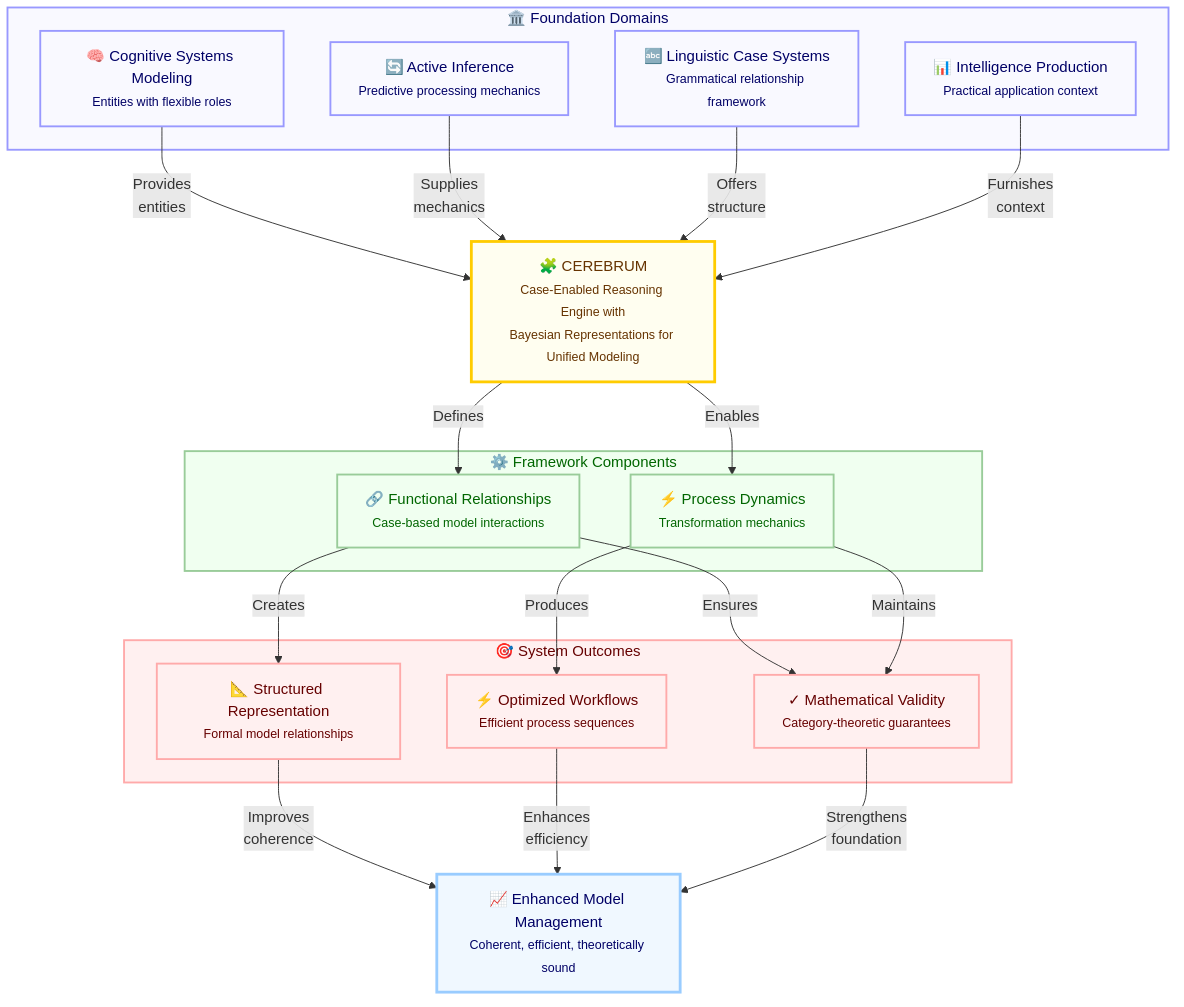
\includegraphics{output/Figure_1.png}
\caption{Foundation Domains of CEREBRUM. The diagram shows the four key
domains (Cognitive Systems Modeling, Active Inference, Linguistic Case
Systems, and Intelligence Production) and their integration through the
CEREBRUM core to produce enhanced model management capabilities.}
\end{figure}

\begin{enumerate}
\def\labelenumi{\arabic{enumi}.}
\tightlist
\item
  \textbf{Cognitive Systems Modeling} offers the entities that take on
  case relationships
\item
  \textbf{Active Inference} supplies the predictive processing mechanics
  that drive case transformations
\item
  \textbf{Linguistic Case Systems} provide the grammatical metaphor for
  how models relate to each other
\item
  \textbf{Intelligence Production} furnishes the practical application
  context and workflows
\end{enumerate}

\hypertarget{methods-and-materials}{%
\section{Methods and Materials}\label{methods-and-materials}}

\hypertarget{formal-framework-development}{%
\subsection{Formal Framework
Development}\label{formal-framework-development}}

The CEREBRUM framework was developed as a part of a broader synthetic
intelligence framework, combining linguistic theory, cognitive science,
category theory, and operations research. Key methodological approaches
included:

\begin{enumerate}
\def\labelenumi{\arabic{enumi}.}
\tightlist
\item
  \textbf{Linguistic Formalization}: Adapting morphosyntactic case
  theory into computational representations through abstract algebraic
  structures.
\item
  \textbf{Category-Theoretic Mapping}: Implementing category theory to
  formalize morphisms between case states as functorial transformations.
\item
  \textbf{Algorithmic Implementation}: Developing algorithmic
  specifications for case transformations compliant with the Free Energy
  Principle.
\item
  \textbf{Variational Methods}: Applying variational free energy
  calculations to optimize model inference as well as structural
  transformations.
\end{enumerate}

\hypertarget{mathematical-foundation}{%
\subsection{Mathematical Foundation}\label{mathematical-foundation}}

The mathematical foundation of CEREBRUM builds on formalizations of case
transformations using category theory and variational inference. Case
transformations are modeled as morphisms in a category where objects are
models with specific case assignments. The framework employs metrics
including Kullback-Leibler divergence, Fisher information, and Lyapunov
functions to quantify transformation efficacy and system stability. This
approach provides both theoretical guarantees of compositional
consistency and practical optimization methods for computational
implementation.

\hypertarget{core-concept-cognitive-models-as-case-bearing-entities}{%
\section{Core Concept: Cognitive Models as Case-Bearing
Entities}\label{core-concept-cognitive-models-as-case-bearing-entities}}

Just as nouns in morphologically rich languages take different forms
based on their grammatical function, cognitive models in CEREBRUM can
exist in different ``states'' or ``cases'' depending on how they relate
to other models or processes within the system. Figure 2 illustrates
this linguistic parallel.

\begin{figure}
\centering
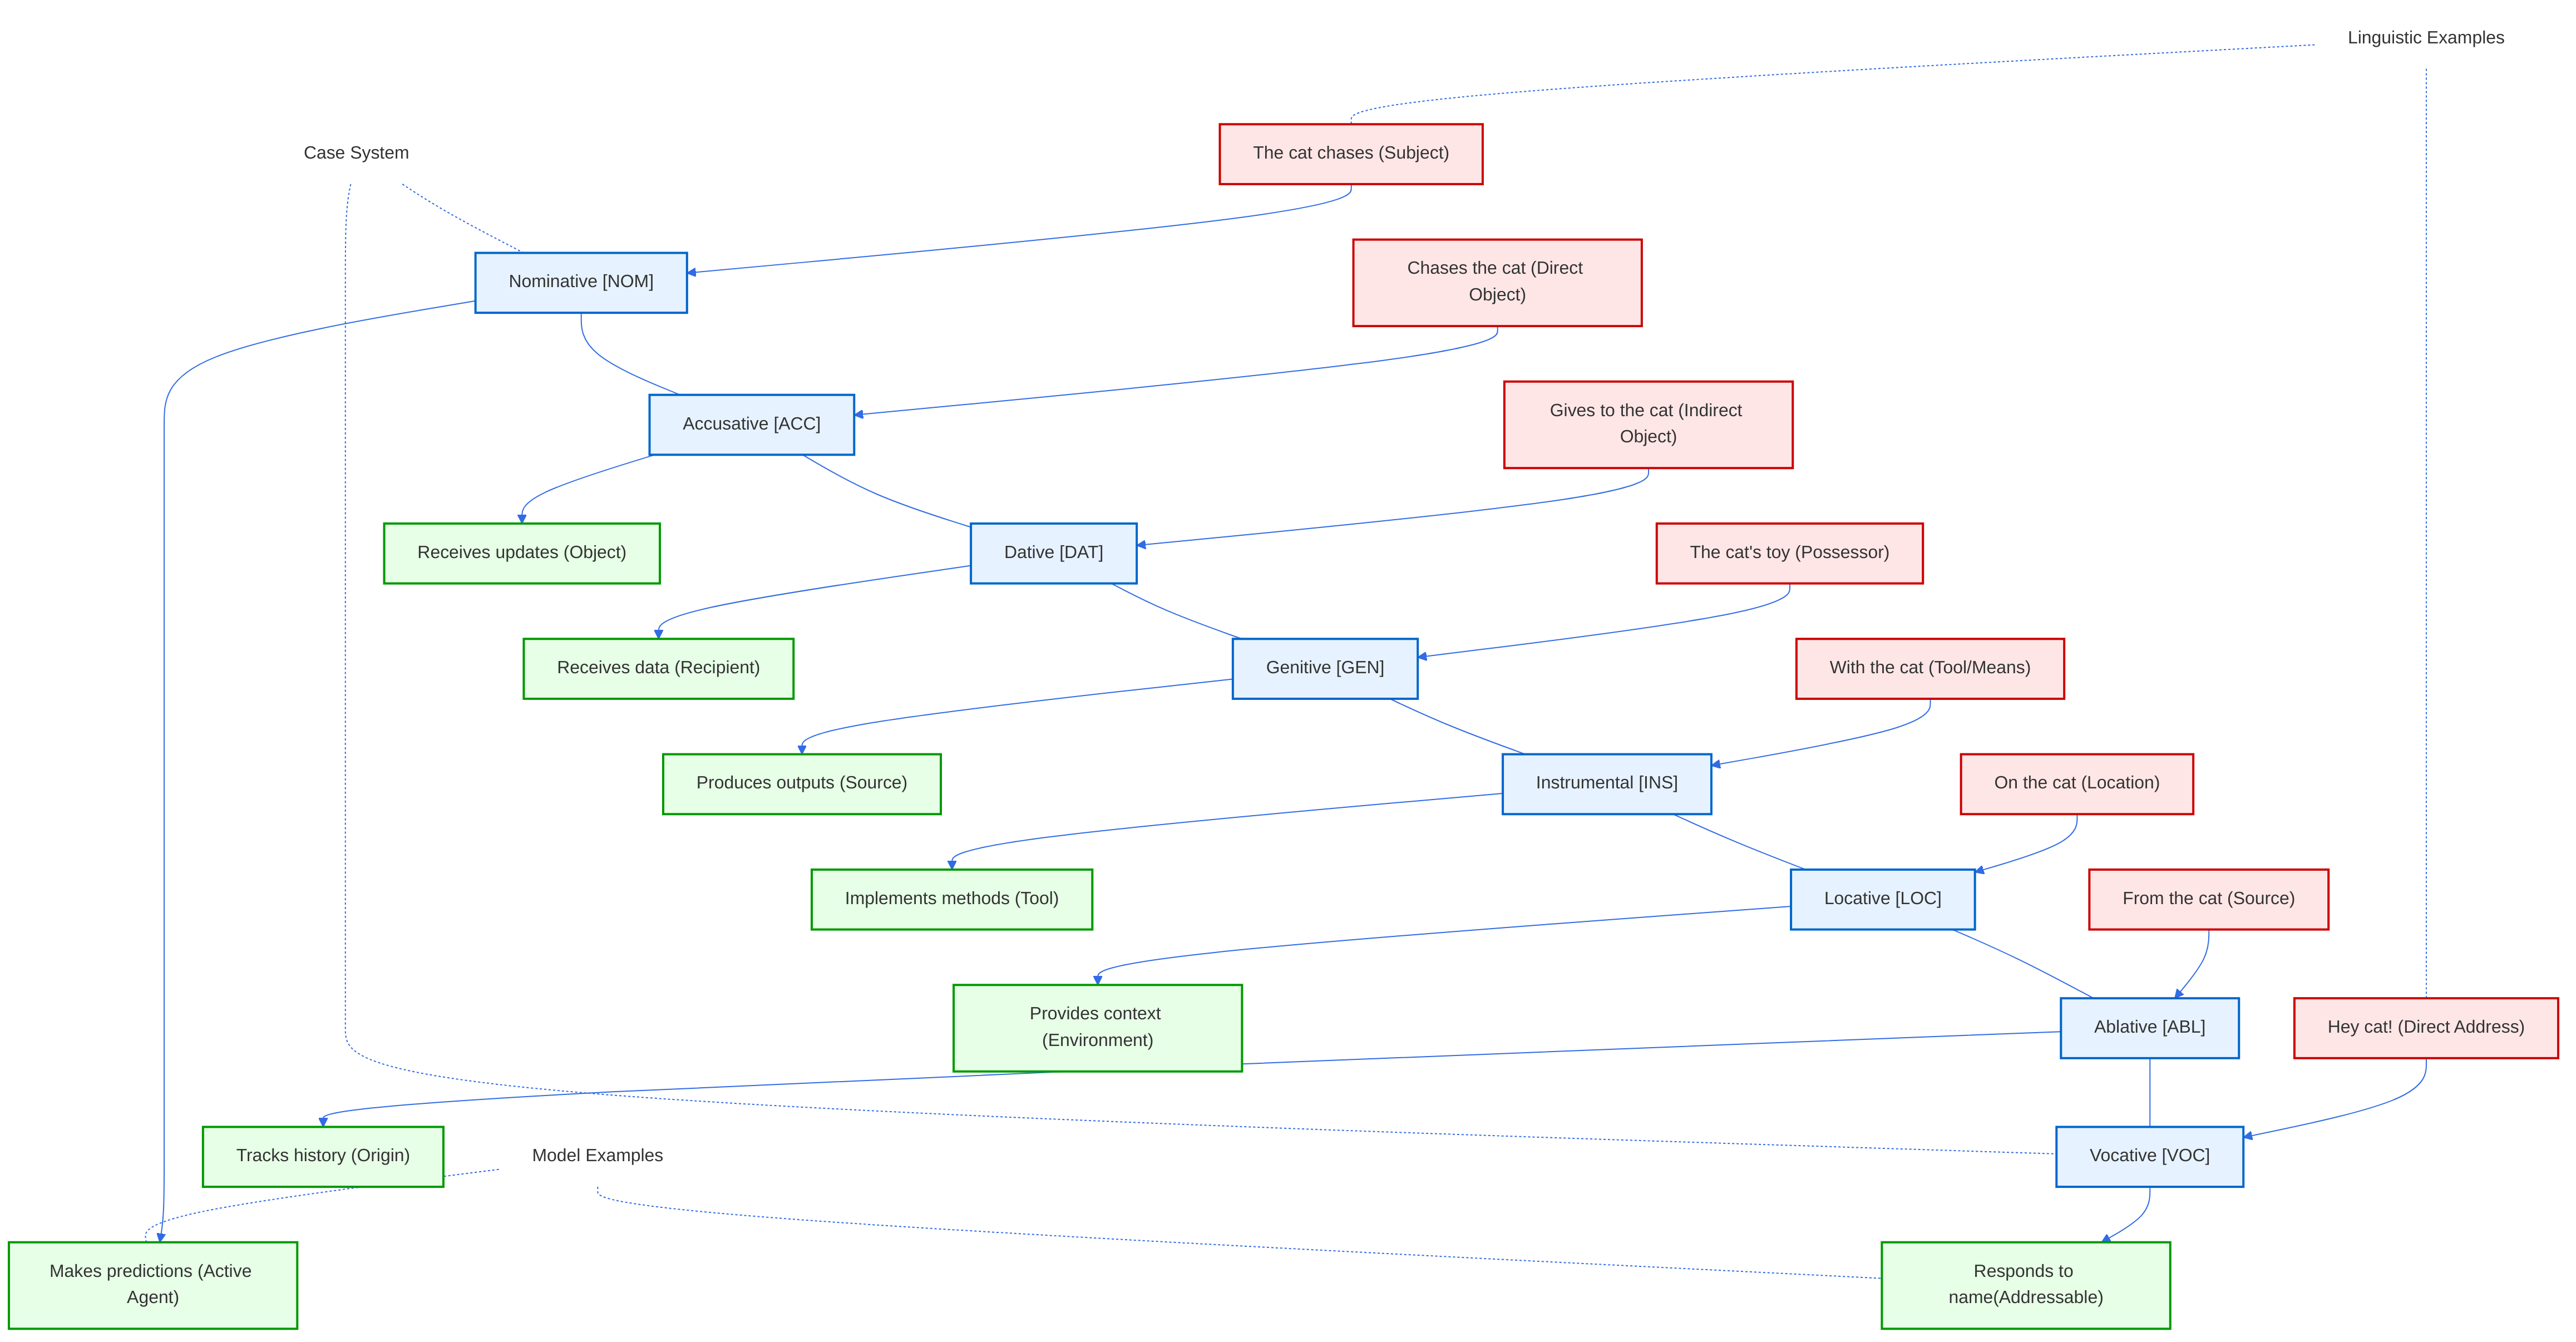
\includegraphics{output/Figure_2.png}
\caption{Case Relationships - Model and Linguistic Parallels. The
diagram illustrates parallel case relationships between a generative
model and linguistic examples, demonstrating how model cases mirror
grammatical roles in natural language.}
\end{figure}

\hypertarget{case-functions-in-cognitive-modeling}{%
\section{Case Functions in Cognitive
Modeling}\label{case-functions-in-cognitive-modeling}}

Each case defines a specific relationship type between models or between
models and data (Table 1). The basic framework is depicted in Figure 3.

\begin{figure}
\centering
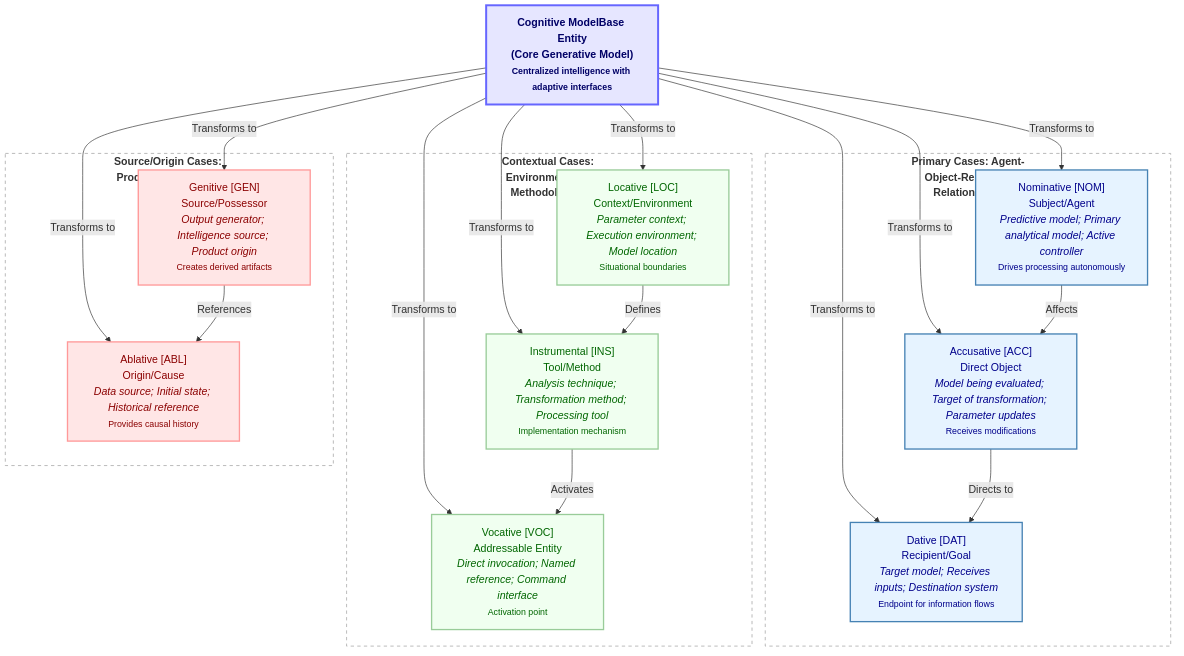
\includegraphics{output/Figure_3.png}
\caption{Cognitive Model Case Framework. The hierarchical organization
of case types in CEREBRUM, showing primary, source, and contextual
declensions with their functional relationships to the core generative
model.}
\end{figure}

\textbf{Table 1: Case Functions in Cognitive Model Systems}

\begin{longtable}[]{@{}llll@{}}
\toprule
\begin{minipage}[b]{0.11\columnwidth}\raggedright
Abbr\strut
\end{minipage} & \begin{minipage}[b]{0.11\columnwidth}\raggedright
Case\strut
\end{minipage} & \begin{minipage}[b]{0.40\columnwidth}\raggedright
Function in CEREBRUM\strut
\end{minipage} & \begin{minipage}[b]{0.27\columnwidth}\raggedright
Example Usage\strut
\end{minipage}\tabularnewline
\midrule
\endhead
\begin{minipage}[t]{0.11\columnwidth}\raggedright
\textbf{{[}NOM{]}}\strut
\end{minipage} & \begin{minipage}[t]{0.11\columnwidth}\raggedright
\textbf{Nominative}\strut
\end{minipage} & \begin{minipage}[t]{0.40\columnwidth}\raggedright
Model as active agent; acts as the primary producer of predictions and
exerts causal influence on other models\strut
\end{minipage} & \begin{minipage}[t]{0.27\columnwidth}\raggedright
Model X {[}NOM{]} generates predictions about data distributions;
controls downstream processing\strut
\end{minipage}\tabularnewline
\begin{minipage}[t]{0.11\columnwidth}\raggedright
\textbf{{[}ACC{]}}\strut
\end{minipage} & \begin{minipage}[t]{0.11\columnwidth}\raggedright
\textbf{Accusative}\strut
\end{minipage} & \begin{minipage}[t]{0.40\columnwidth}\raggedright
Model as object of process; receives transformations and updates from
other models or processes\strut
\end{minipage} & \begin{minipage}[t]{0.27\columnwidth}\raggedright
Process applies to Model X {[}ACC{]}; optimization procedures refine
Model X's parameters\strut
\end{minipage}\tabularnewline
\begin{minipage}[t]{0.11\columnwidth}\raggedright
\textbf{{[}GEN{]}}\strut
\end{minipage} & \begin{minipage}[t]{0.11\columnwidth}\raggedright
\textbf{Genitive}\strut
\end{minipage} & \begin{minipage}[t]{0.40\columnwidth}\raggedright
Model as source/possessor; functions as the origin of outputs, products,
and derived models\strut
\end{minipage} & \begin{minipage}[t]{0.27\columnwidth}\raggedright
Output of Model X {[}GEN{]}; intelligence products derived from Model
X's inferences\strut
\end{minipage}\tabularnewline
\begin{minipage}[t]{0.11\columnwidth}\raggedright
\textbf{{[}DAT{]}}\strut
\end{minipage} & \begin{minipage}[t]{0.11\columnwidth}\raggedright
\textbf{Dative}\strut
\end{minipage} & \begin{minipage}[t]{0.40\columnwidth}\raggedright
Model as recipient; specifically configured to receive and process
incoming data flows\strut
\end{minipage} & \begin{minipage}[t]{0.27\columnwidth}\raggedright
Data fed into Model X {[}DAT{]}; Model X receives information from
external sources\strut
\end{minipage}\tabularnewline
\begin{minipage}[t]{0.11\columnwidth}\raggedright
\textbf{{[}INS{]}}\strut
\end{minipage} & \begin{minipage}[t]{0.11\columnwidth}\raggedright
\textbf{Instrumental}\strut
\end{minipage} & \begin{minipage}[t]{0.40\columnwidth}\raggedright
Model as method/tool; serves as the means by which analytical operations
are performed\strut
\end{minipage} & \begin{minipage}[t]{0.27\columnwidth}\raggedright
Analysis performed via Model X {[}INS{]}; Model X implements analytical
procedures\strut
\end{minipage}\tabularnewline
\begin{minipage}[t]{0.11\columnwidth}\raggedright
\textbf{{[}LOC{]}}\strut
\end{minipage} & \begin{minipage}[t]{0.11\columnwidth}\raggedright
\textbf{Locative}\strut
\end{minipage} & \begin{minipage}[t]{0.40\columnwidth}\raggedright
Model as context; provides environmental constraints and situational
parameters\strut
\end{minipage} & \begin{minipage}[t]{0.27\columnwidth}\raggedright
Parameters within Model X {[}LOC{]}; environmental contingencies modeled
by X\strut
\end{minipage}\tabularnewline
\begin{minipage}[t]{0.11\columnwidth}\raggedright
\textbf{{[}ABL{]}}\strut
\end{minipage} & \begin{minipage}[t]{0.11\columnwidth}\raggedright
\textbf{Ablative}\strut
\end{minipage} & \begin{minipage}[t]{0.40\columnwidth}\raggedright
Model as origin/cause; represents historical conditions or causal
precursors\strut
\end{minipage} & \begin{minipage}[t]{0.27\columnwidth}\raggedright
Insights derived from Model X {[}ABL{]}; causal attributions traced to
Model X\strut
\end{minipage}\tabularnewline
\begin{minipage}[t]{0.11\columnwidth}\raggedright
\textbf{{[}VOC{]}}\strut
\end{minipage} & \begin{minipage}[t]{0.11\columnwidth}\raggedright
\textbf{Vocative}\strut
\end{minipage} & \begin{minipage}[t]{0.40\columnwidth}\raggedright
Model as addressable entity; functions as a directly callable interface
with name-based activation\strut
\end{minipage} & \begin{minipage}[t]{0.27\columnwidth}\raggedright
``Hey Model X'' {[}VOC{]}; direct invocation of Model X for task
initialization; documentation reference point\strut
\end{minipage}\tabularnewline
\bottomrule
\end{longtable}

Within intelligence production systems, these case relationships serve
critical functional roles: nominative models act as primary analytical
engines driving the intelligence case; accusative models become targets
of quality assessment and improvement; multimodal genitive models
generate documentation and reports; dative models receive and process
collected intelligence data; instrumental models provide the
methodological framework for investigations; locative models establish
situational boundaries; ablative models represent the historical origins
of analytical conclusions; and vocative models serve as directly
addressable interfaces for command initiation and documentation
reference. Together, these case relationships create a comprehensive
framework for structured intelligence workflows.

Figure 4 illustrates how this core framework integrates with
intelligence case management.

\begin{figure}
\centering
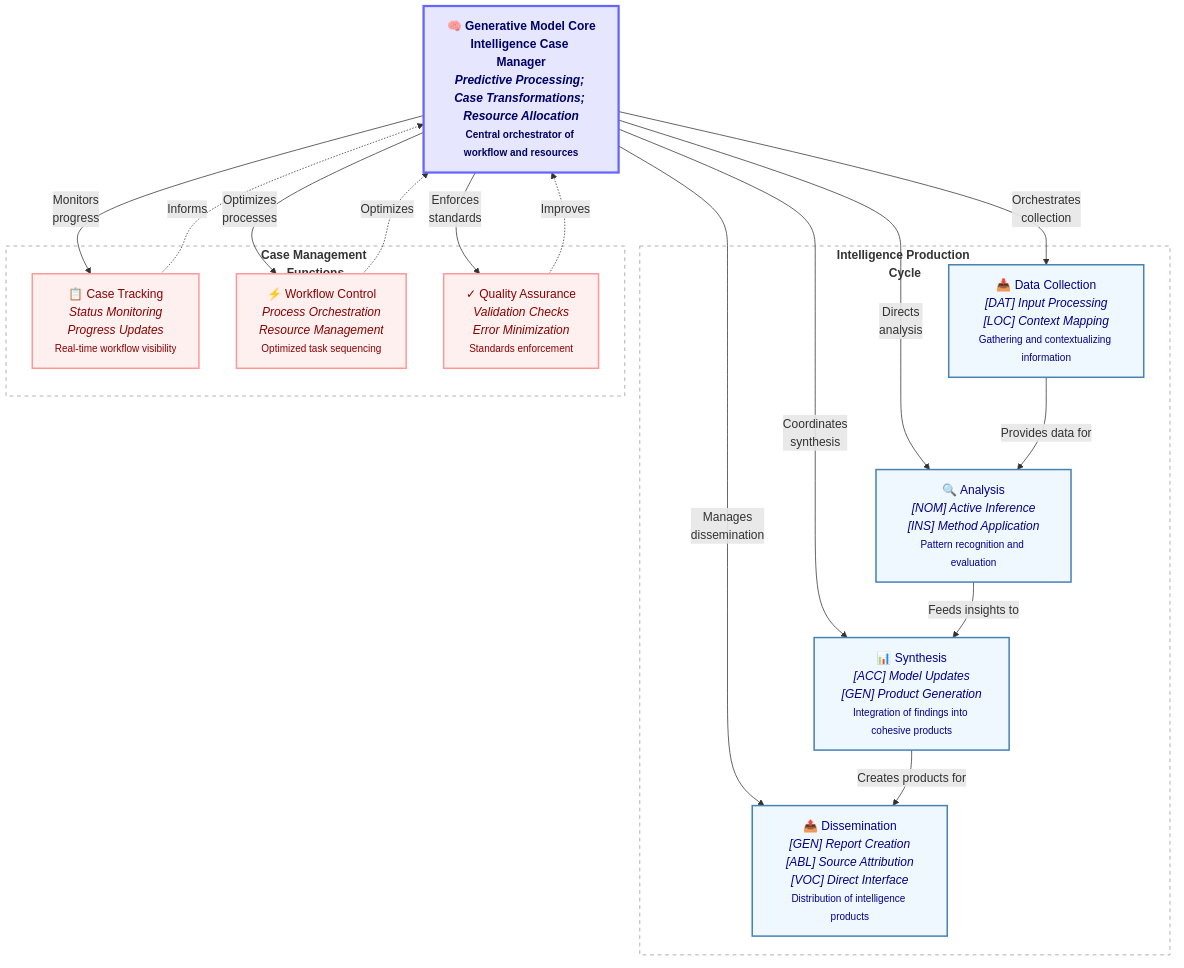
\includegraphics{output/Figure_4.png}
\caption{Generative Model Integration in Intelligence Case Management.
Illustrates how CEREBRUM's generative model core orchestrates
intelligence production and case management through case-specific
transformations.}
\end{figure}

\hypertarget{a-preliminary-example-of-a-case-bearing-model-homeostatic-thermostat}{%
\section{A Preliminary Example of a Case-Bearing Model: Homeostatic
Thermostat}\label{a-preliminary-example-of-a-case-bearing-model-homeostatic-thermostat}}

Consider a cognitive model of a homeostatic thermostat that perceives
room temperature with a thermometer, and regulates temperature through
connected heating and cooling systems. In nominative case {[}NOM{]}, the
thermostat model actively generates temperature predictions and
dispatches control signals, functioning as the primary agent in the
temperature regulation process. When placed in accusative case
{[}ACC{]}, this same model becomes the object of optimization processes,
with its parameters being updated based on prediction errors between
expected and actual temperature readings. In dative case {[}DAT{]}, the
thermostat model receives environmental temperature data streams and
occupant comfort preferences as inputs. The genitive case {[}GEN{]}
transforms the model into a generator of temperature regulation reports
and system performance analytics (``genitive AI''). When in instrumental
case {[}INS{]}, the thermostat serves as a computational tool
implementing control algorithms for other systems requiring temperature
management. The locative case {[}LOC{]} reconfigures the model to
represent the contextual environment in which temperature regulation
occurs, modeling building thermal properties, or discussing something
within the model as a location. Finally, in ablative case {[}ABL{]}, the
thermostat functions as the origin of historical temperature data and
control decisions, providing causal explanations for current thermal
conditions. This single cognitive model thus assumes dramatically
different functional roles while maintaining its core identity as a
thermostat.

\hypertarget{declinability-of-active-inference-generative-models}{%
\section{Declinability of Active Inference Generative
Models}\label{declinability-of-active-inference-generative-models}}

At the core of CEREBRUM lies the concept of \textbf{declinability} - the
capacity for generative models to assume different morphological and
functional roles through case transformations, mirroring the declension
patterns of nouns in morphologically rich languages. Unlike traditional
approaches where models maintain fixed roles, or variable roles defined
by analytical pipelines, CEREBRUM treats cognitive models as flexible
entities capable of morphological adaptation to different operational
contexts.

\hypertarget{morphological-transformation-of-generative-models}{%
\subsection{Morphological Transformation of Generative
Models}\label{morphological-transformation-of-generative-models}}

When an active inference generative model undergoes case transformation,
it experiences orchestrated systematic changes summarized in Table 2:

\begin{enumerate}
\def\labelenumi{\arabic{enumi}.}
\tightlist
\item
  \textbf{Functional Interfaces}: Input/output specifications change to
  match the case role requirements
\item
  \textbf{Parameter Access Patterns}: Which parameters are exposed or
  constrained changes based on case
\item
  \textbf{Prior Distributions}: Different cases employ different prior
  constraints on parameter values
\item
  \textbf{Update Dynamics}: The ways in which the model updates its
  internal states vary by case role
\item
  \textbf{Computational Resources}: Different cases receive different
  precision-weighted computational allocations
\end{enumerate}

\textbf{Table 2: Transformational Properties of Active Inference
Generative Models Under Case Declensions}

\begin{longtable}[]{@{}llll@{}}
\toprule
\begin{minipage}[b]{0.08\columnwidth}\raggedright
Case\strut
\end{minipage} & \begin{minipage}[b]{0.24\columnwidth}\raggedright
Parametric Changes\strut
\end{minipage} & \begin{minipage}[b]{0.33\columnwidth}\raggedright
Interface Transformations\strut
\end{minipage} & \begin{minipage}[b]{0.24\columnwidth}\raggedright
Precision Weighting\strut
\end{minipage}\tabularnewline
\midrule
\endhead
\begin{minipage}[t]{0.08\columnwidth}\raggedright
\textbf{{[}NOM{]}}\strut
\end{minipage} & \begin{minipage}[t]{0.24\columnwidth}\raggedright
Fully accessible parameters; all degrees of freedom available for
prediction generation; strongest prior constraints on likelihood
mapping\strut
\end{minipage} & \begin{minipage}[t]{0.33\columnwidth}\raggedright
Outputs predictions; exposes forward inference pathways; prediction
interfaces activated\strut
\end{minipage} & \begin{minipage}[t]{0.24\columnwidth}\raggedright
Highest precision on likelihood; maximizes precision of generative
mapping from internal states to observations\strut
\end{minipage}\tabularnewline
\begin{minipage}[t]{0.08\columnwidth}\raggedright
\textbf{{[}ACC{]}}\strut
\end{minipage} & \begin{minipage}[t]{0.24\columnwidth}\raggedright
Restricted parameter access; plasticity gates opened; learning rate
parameters prioritized\strut
\end{minipage} & \begin{minipage}[t]{0.33\columnwidth}\raggedright
Receives transformations; update interfaces exposed; gradient reception
pathways active\strut
\end{minipage} & \begin{minipage}[t]{0.24\columnwidth}\raggedright
Highest precision on parameters; maximizes precision of parameter
updates based on prediction errors\strut
\end{minipage}\tabularnewline
\begin{minipage}[t]{0.08\columnwidth}\raggedright
\textbf{{[}DAT{]}}\strut
\end{minipage} & \begin{minipage}[t]{0.24\columnwidth}\raggedright
Input-focused parameterization; sensory mapping parameters prioritized;
perceptual categorization parameters activated\strut
\end{minipage} & \begin{minipage}[t]{0.33\columnwidth}\raggedright
Receives data flows; input processing interfaces exposed; sensory
reception channels active\strut
\end{minipage} & \begin{minipage}[t]{0.24\columnwidth}\raggedright
Highest precision on inputs; maximizes precision of incoming data
relative to internal expectations\strut
\end{minipage}\tabularnewline
\begin{minipage}[t]{0.08\columnwidth}\raggedright
\textbf{{[}GEN{]}}\strut
\end{minipage} & \begin{minipage}[t]{0.24\columnwidth}\raggedright
``Genitive AI''; Output-focused parameterization; production parameters
activated; generative pathway emphasis\strut
\end{minipage} & \begin{minipage}[t]{0.33\columnwidth}\raggedright
Generates products; output interfaces prioritized; production pathways
activated\strut
\end{minipage} & \begin{minipage}[t]{0.24\columnwidth}\raggedright
Highest precision on outputs; maximizes precision of generated products
relative to internal models\strut
\end{minipage}\tabularnewline
\begin{minipage}[t]{0.08\columnwidth}\raggedright
\textbf{{[}INS{]}}\strut
\end{minipage} & \begin{minipage}[t]{0.24\columnwidth}\raggedright
Method-oriented parameters exposed; algorithmic parameters accessible;
procedural knowledge emphasized\strut
\end{minipage} & \begin{minipage}[t]{0.33\columnwidth}\raggedright
Implements processes; computational interfaces active; procedural
execution pathways open\strut
\end{minipage} & \begin{minipage}[t]{0.24\columnwidth}\raggedright
Highest precision on operations; maximizes precision of procedural
execution relative to methodological expectations\strut
\end{minipage}\tabularnewline
\begin{minipage}[t]{0.08\columnwidth}\raggedright
\textbf{{[}LOC{]}}\strut
\end{minipage} & \begin{minipage}[t]{0.24\columnwidth}\raggedright
Context parameters emphasized; environmental modeling parameters
prioritized; situational knowledge emphasized\strut
\end{minipage} & \begin{minipage}[t]{0.33\columnwidth}\raggedright
Provides environmental constraints; contextual interfaces active;
environmental modeling pathways prioritized\strut
\end{minipage} & \begin{minipage}[t]{0.24\columnwidth}\raggedright
Highest precision on contexts; maximizes precision of contextual
representation relative to environmental dynamics\strut
\end{minipage}\tabularnewline
\begin{minipage}[t]{0.08\columnwidth}\raggedright
\textbf{{[}ABL{]}}\strut
\end{minipage} & \begin{minipage}[t]{0.24\columnwidth}\raggedright
Origin states emphasized; historical parameters accessible; causal
attribution pathways strengthened\strut
\end{minipage} & \begin{minipage}[t]{0.33\columnwidth}\raggedright
Source of information; historical data interfaces active; causal
explanation pathways open\strut
\end{minipage} & \begin{minipage}[t]{0.24\columnwidth}\raggedright
Highest precision on historical data; maximizes precision of causal
attributions and historical reconstructions\strut
\end{minipage}\tabularnewline
\begin{minipage}[t]{0.08\columnwidth}\raggedright
\textbf{{[}VOC{]}}\strut
\end{minipage} & \begin{minipage}[t]{0.24\columnwidth}\raggedright
Identity parameters prioritized; naming and identification parameters
activated; interface exposure emphasized\strut
\end{minipage} & \begin{minipage}[t]{0.33\columnwidth}\raggedright
Maintains addressable interfaces; name recognition pathways activated;
command reception channels open\strut
\end{minipage} & \begin{minipage}[t]{0.24\columnwidth}\raggedright
Highest precision on identification cues; maximizes precision of name
recognition relative to calling patterns\strut
\end{minipage}\tabularnewline
\bottomrule
\end{longtable}

\hypertarget{active-inference-model-declension-example}{%
\subsection{Active Inference Model Declension
Example}\label{active-inference-model-declension-example}}

Consider a perception-oriented generative model M with parameters theta,
internal states s, and observational distribution p(o\textbar s,theta).
When declined across cases, this single model transforms as follows:

\begin{itemize}
\tightlist
\item
  \textbf{M{[}NOM{]}}: Actively generates predictions by sampling from
  p(o\textbar s,theta), with all parameters fully accessible
\item
  \textbf{M{[}ACC{]}}: Becomes the target of updates, with parameter
  gradients calculated from prediction errors
\item
  \textbf{M{[}DAT{]}}: Configured to receive data flows, with specific
  input interfaces activated
\item
  \textbf{M{[}GEN{]}}: Optimized to generate outputs, with output
  interfaces prioritized
\item
  \textbf{M{[}INS{]}}: Functions as a computational method, exposing
  algorithmic interfaces
\item
  \textbf{M{[}LOC{]}}: Provides contextual constraints for other models,
  with environmental parameters exposed
\item
  \textbf{M{[}ABL{]}}: Serves as an information source, with historical
  data accessible
\item
  \textbf{M{[}VOC{]}}: Functions as an addressable entity responding to
  direct invocation, with naming parameters activated
\end{itemize}

The Vocative case {[}VOC{]} represents a unique functional role where
models serve as directly addressable entities within a model ecosystem.
Unlike other cases that focus on data processing or transformational
aspects, the vocative case specifically optimizes a model for name-based
recognition and command reception. This has particular relevance in
synthetic intelligence environments where models must be selectively
activated or ``woken up'' through explicit address, similar to how
humans are called by name to gain their attention. The vocative case
maintains specialized interfaces for handling direct commands,
documentation references, and initialization requests. In practical
applications, models in vocative case might serve as conversational
agents awaiting activation, documentation reference points within
technical specifications, or system components that remain dormant until
explicitly addressed. This pattern mimics the linguistic vocative case
where a noun is used in direct address, as in ``Hey Siri'' or ``OK
Google'' activation phrases for digital assistants, creating a natural
bridging pattern between human language interaction and model
orchestration.

This systematic pattern of transformations constitutes a complete
``declension paradigm'' for cognitive models, using precision-modulation
to fulfill diverse functional roles while maintaining their core
identity.

\hypertarget{model-workflows-as-case-transformations}{%
\section{Model Workflows as Case
Transformations}\label{model-workflows-as-case-transformations}}

Case transformations represent operations that change the functional
role of a model in the system, reflecting active inference principles of
prediction and error minimization. Figure 5 provides a sequence diagram
of a typical transformation cycle, and Figure 6 shows the intelligence
production workflow where these transformations occur.

\begin{figure}
\centering
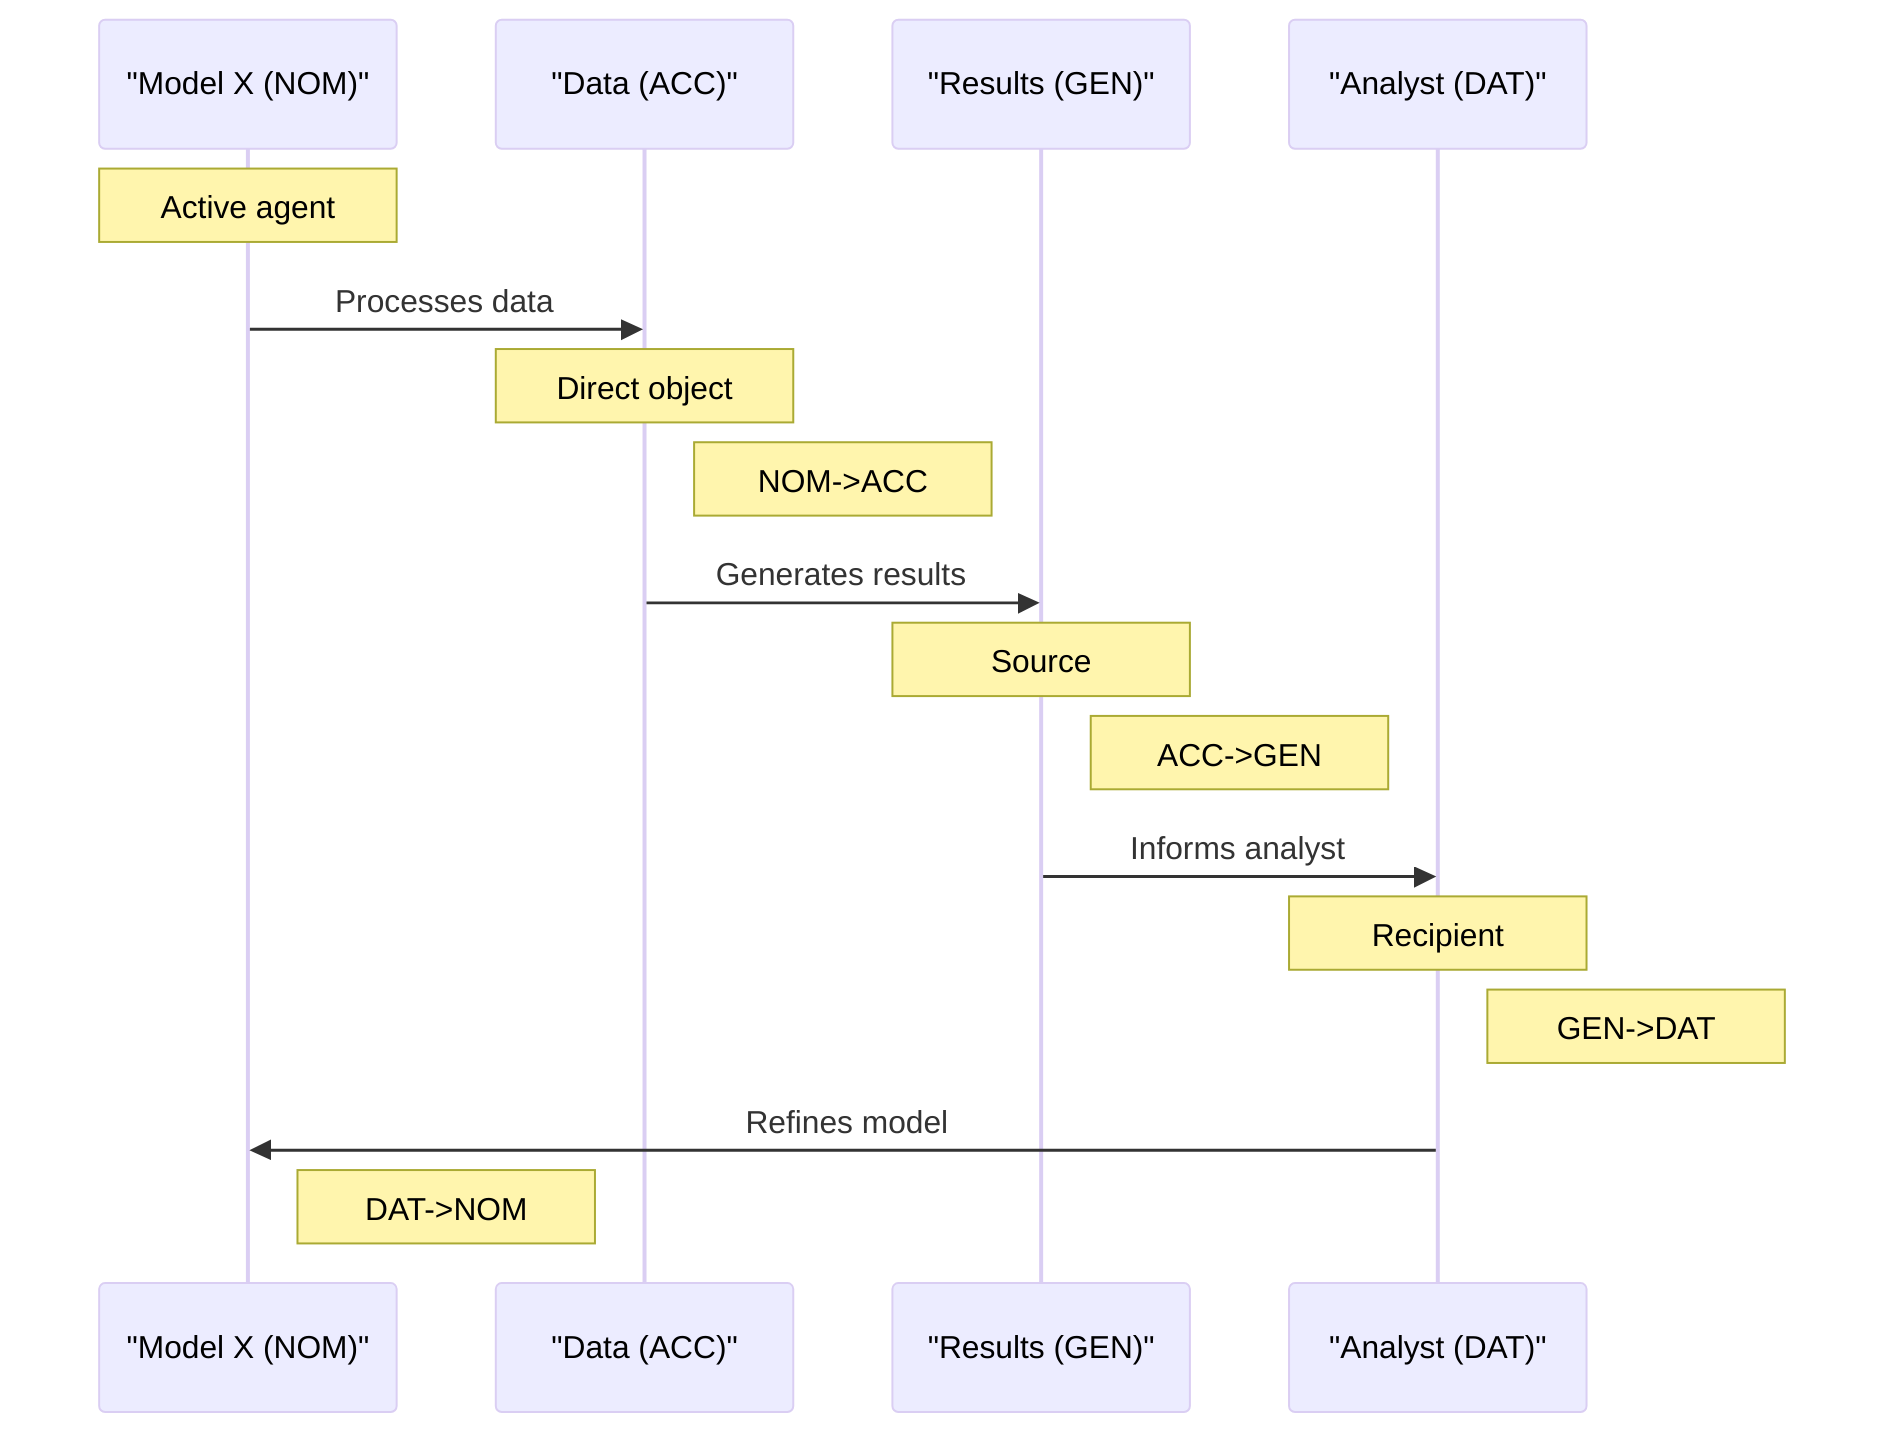
\includegraphics{output/Figure_5.png}
\caption{Model Workflows as Case Transformations - Sequence Diagram 1.
Illustrates the temporal sequence of case transformations as models
transition through different functional roles in an intelligence
workflow.}
\end{figure}

\begin{figure}
\centering
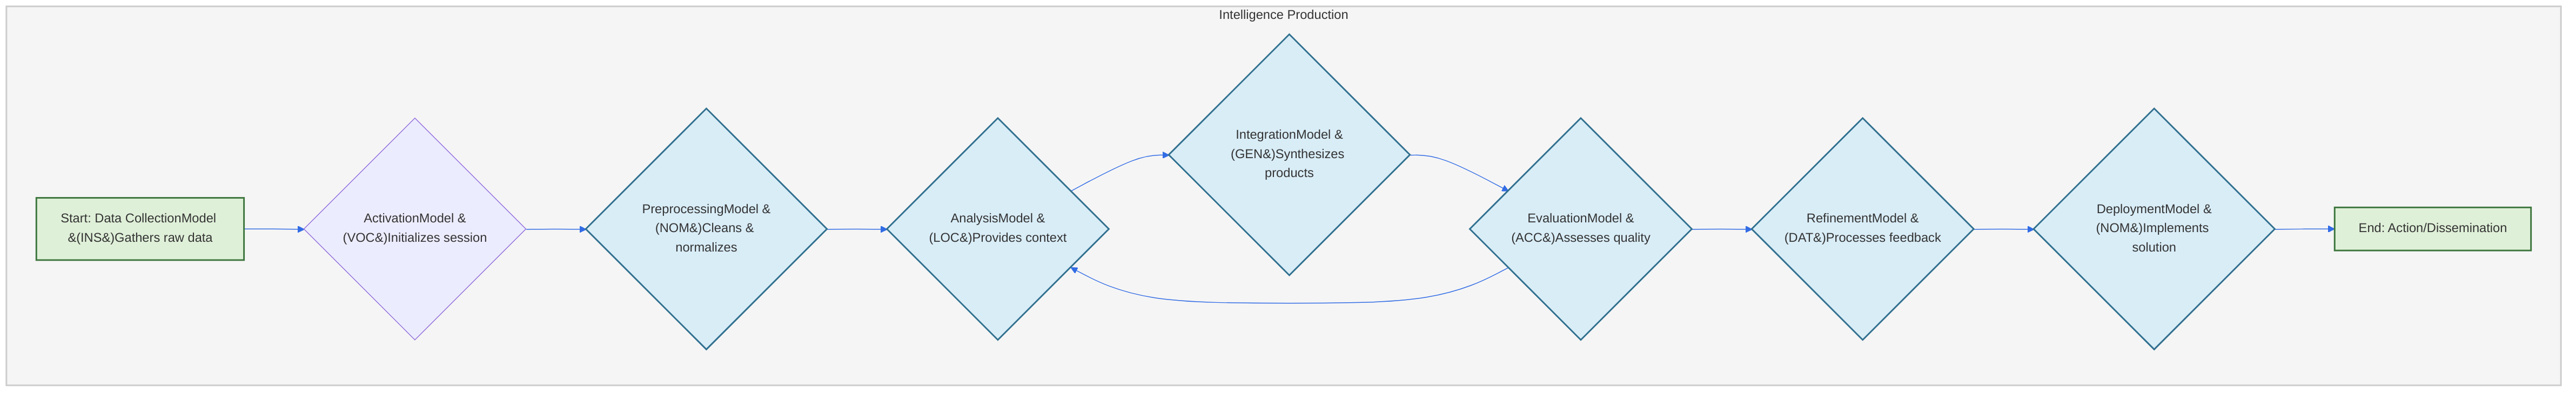
\includegraphics{output/Figure_6.png}
\caption{Intelligence Production Workflow with Case-Bearing Models.
Illustrates the intelligence production cycle, showing the stages where
models with different case assignments participate.}
\end{figure}

\hypertarget{category-theoretic-formalization}{%
\section{Category-Theoretic
Formalization}\label{category-theoretic-formalization}}

CEREBRUM employs category theory to formalize case relationships between
cognitive models, creating a rigorous mathematical foundation,
illustrated in Figure 7 and Figure 8.

\begin{figure}
\centering
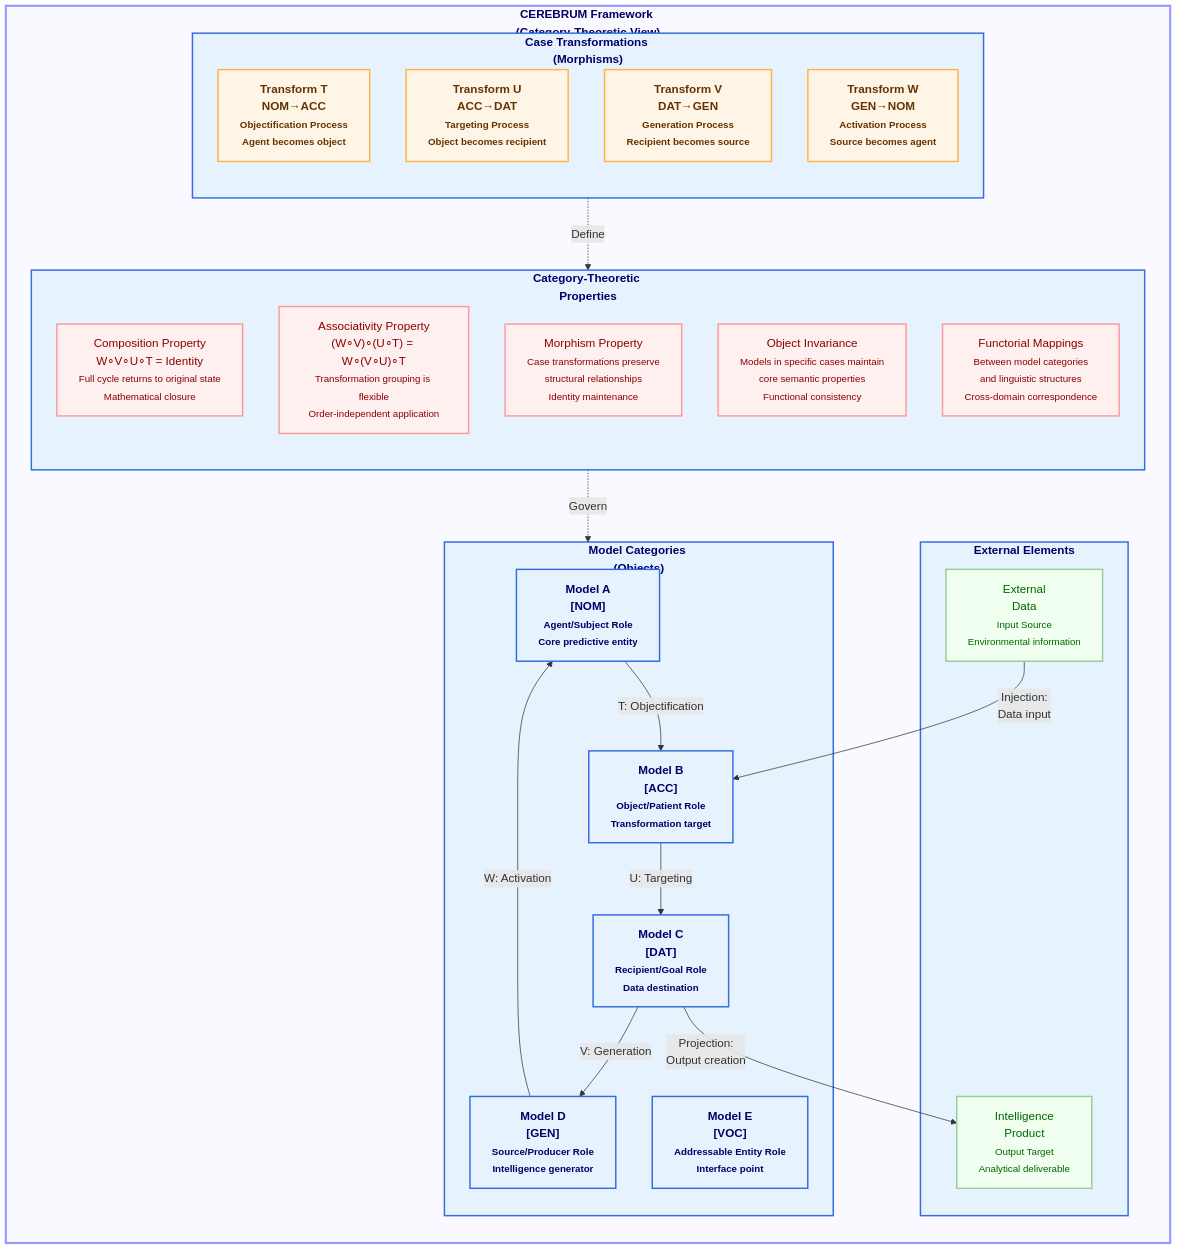
\includegraphics{output/Figure_7.png}
\caption{CEREBRUM Category Theory Framework. Demonstrates the
category-theoretic formalization of case relationships and
transformations between cognitive models.}
\end{figure}

\begin{figure}
\centering
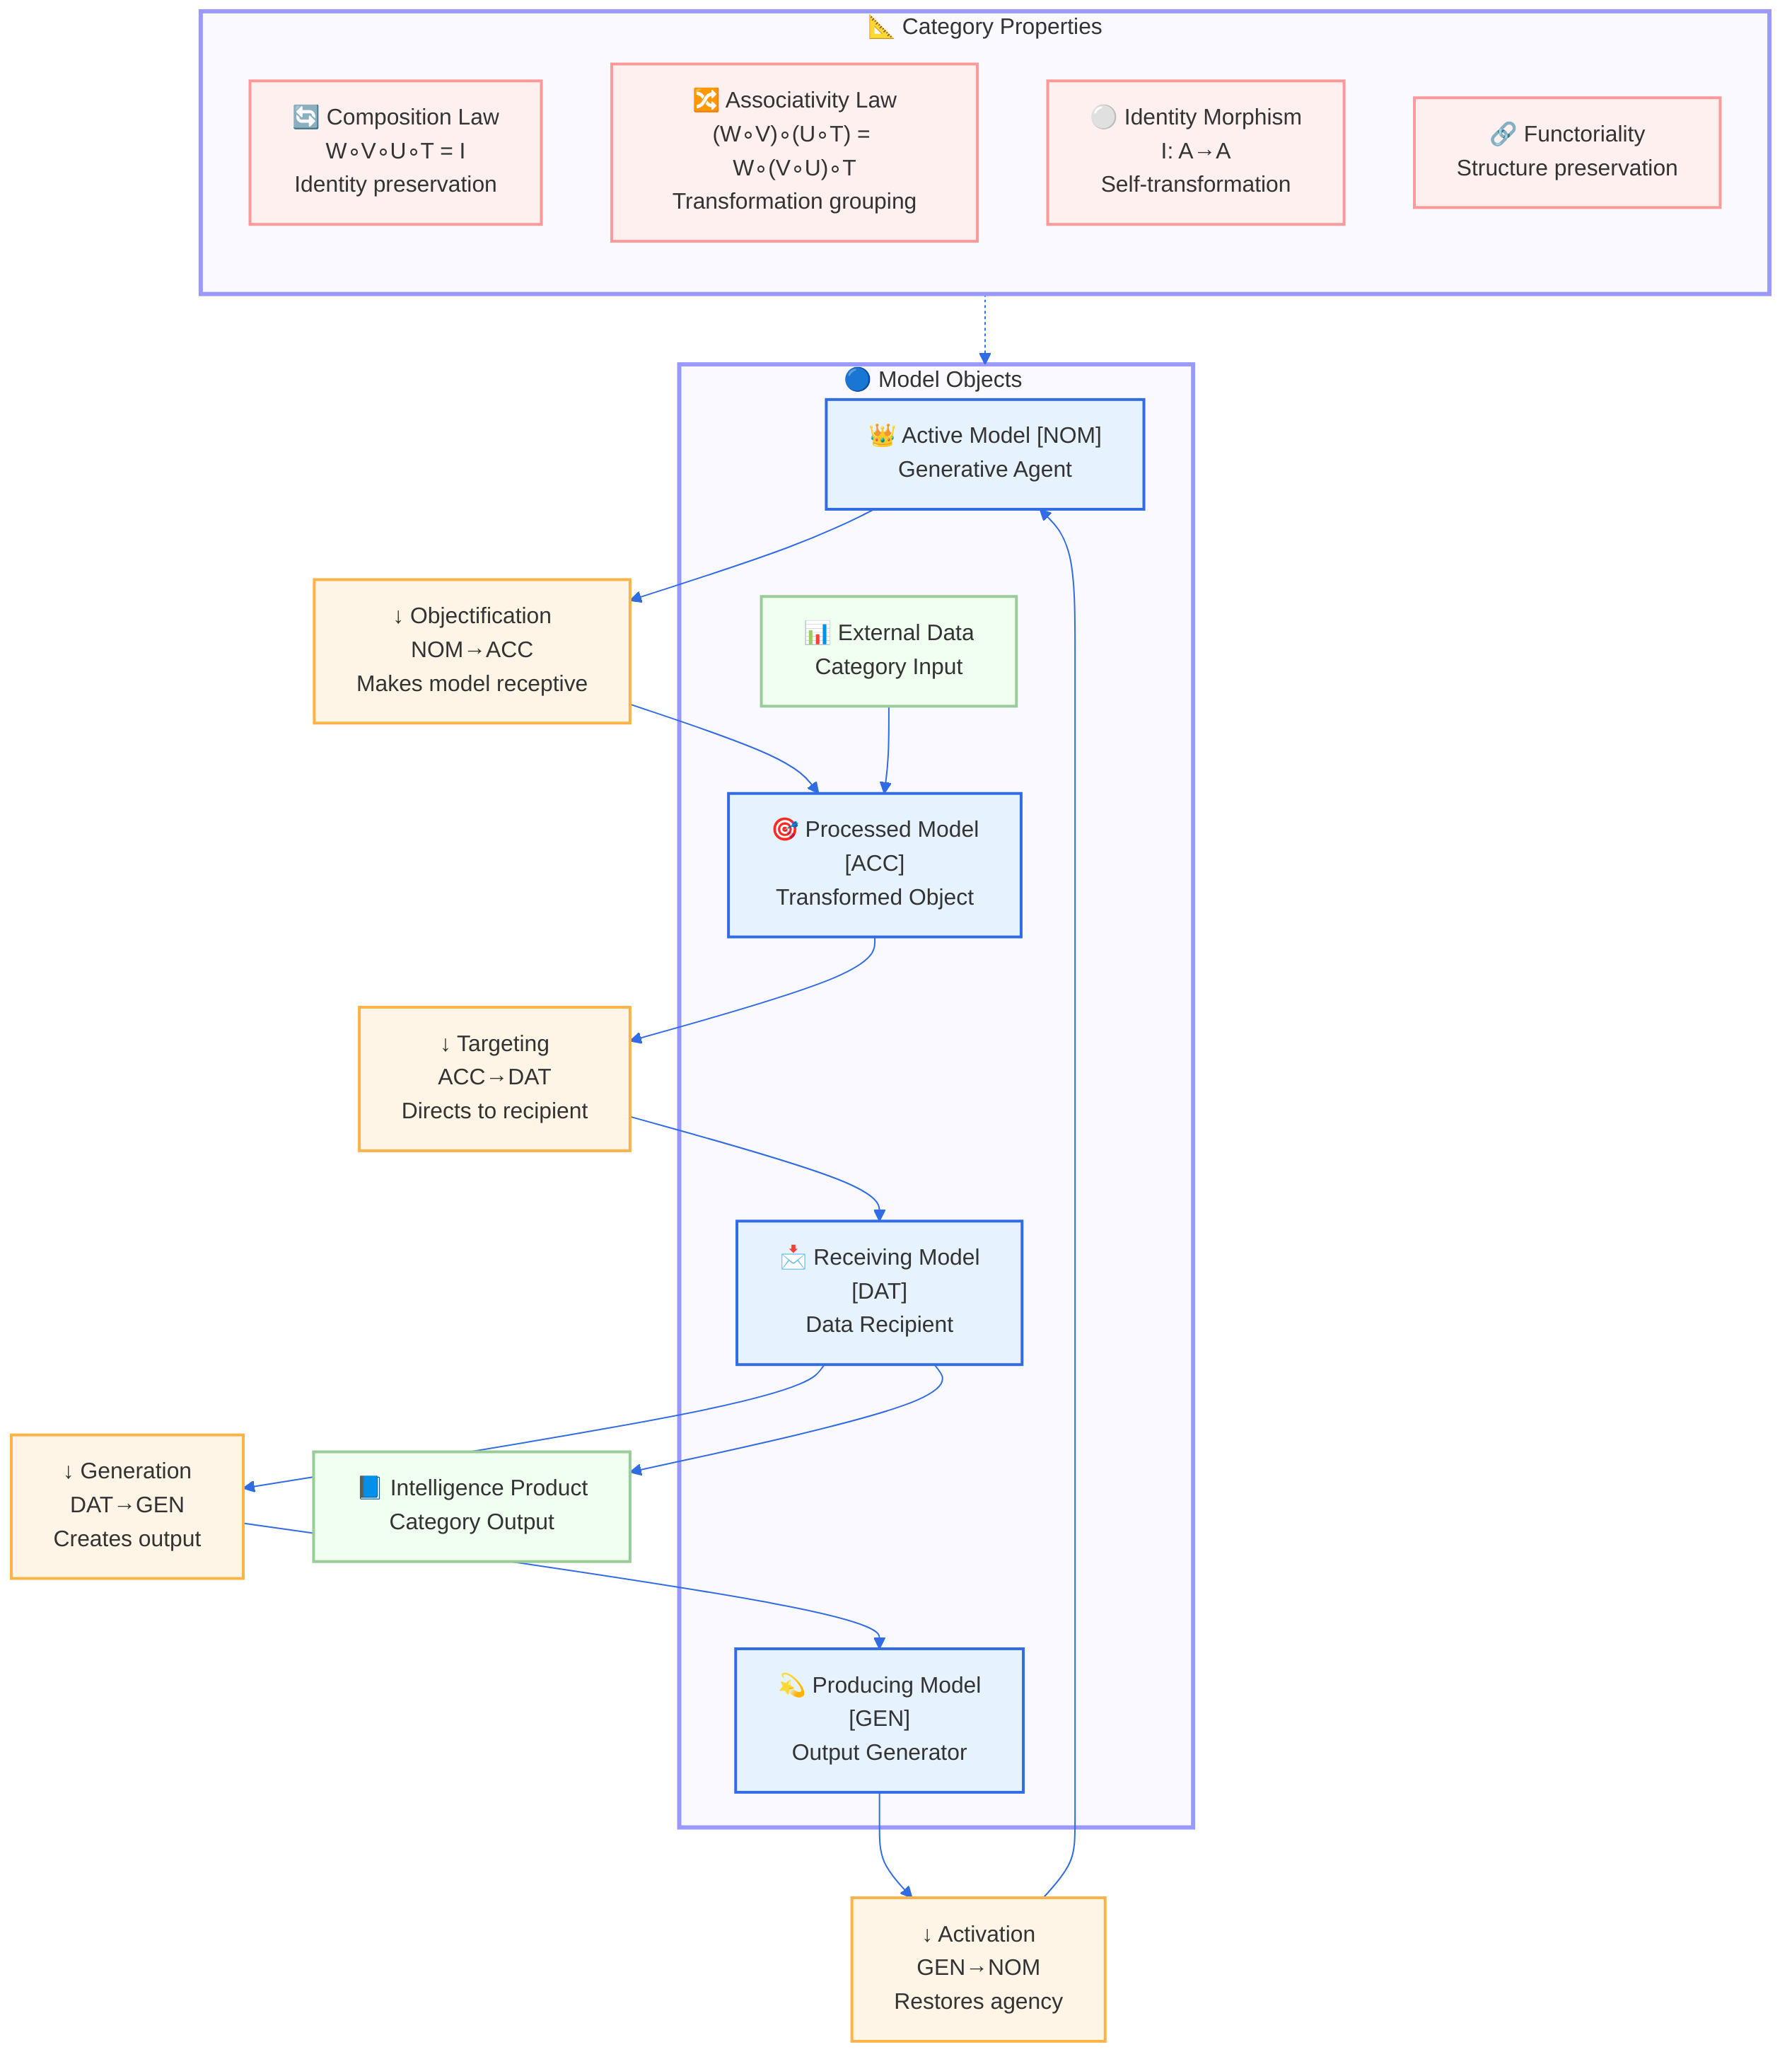
\includegraphics{output/Figure_8.png}
\caption{Category Theory Framework (Alternative View). Further
illustrates the category-theoretic components and properties within
CEREBRUM.}
\end{figure}

\hypertarget{computational-linguistics-structural-alignment-and-model-relationships}{%
\section{Computational Linguistics, Structural Alignment, and Model
Relationships}\label{computational-linguistics-structural-alignment-and-model-relationships}}

CEREBRUM supports different alignment systems for model relationships,
mirroring linguistic morphosyntactic structures (Figure 9). These
alignment patterns determine how models interact and transform based on
their functional roles. Figure 9 illustrates the core alignment patterns
derived from linguistic theory, showing how models can be organized
based on their case relationships. This includes nominative-accusative
alignment (where models are distinguished by their role as agents or
patients), ergative-absolutive alignment (where models are grouped by
their relationship to actions), and tripartite alignment (where each
case is marked distinctly).

\begin{figure}
\centering
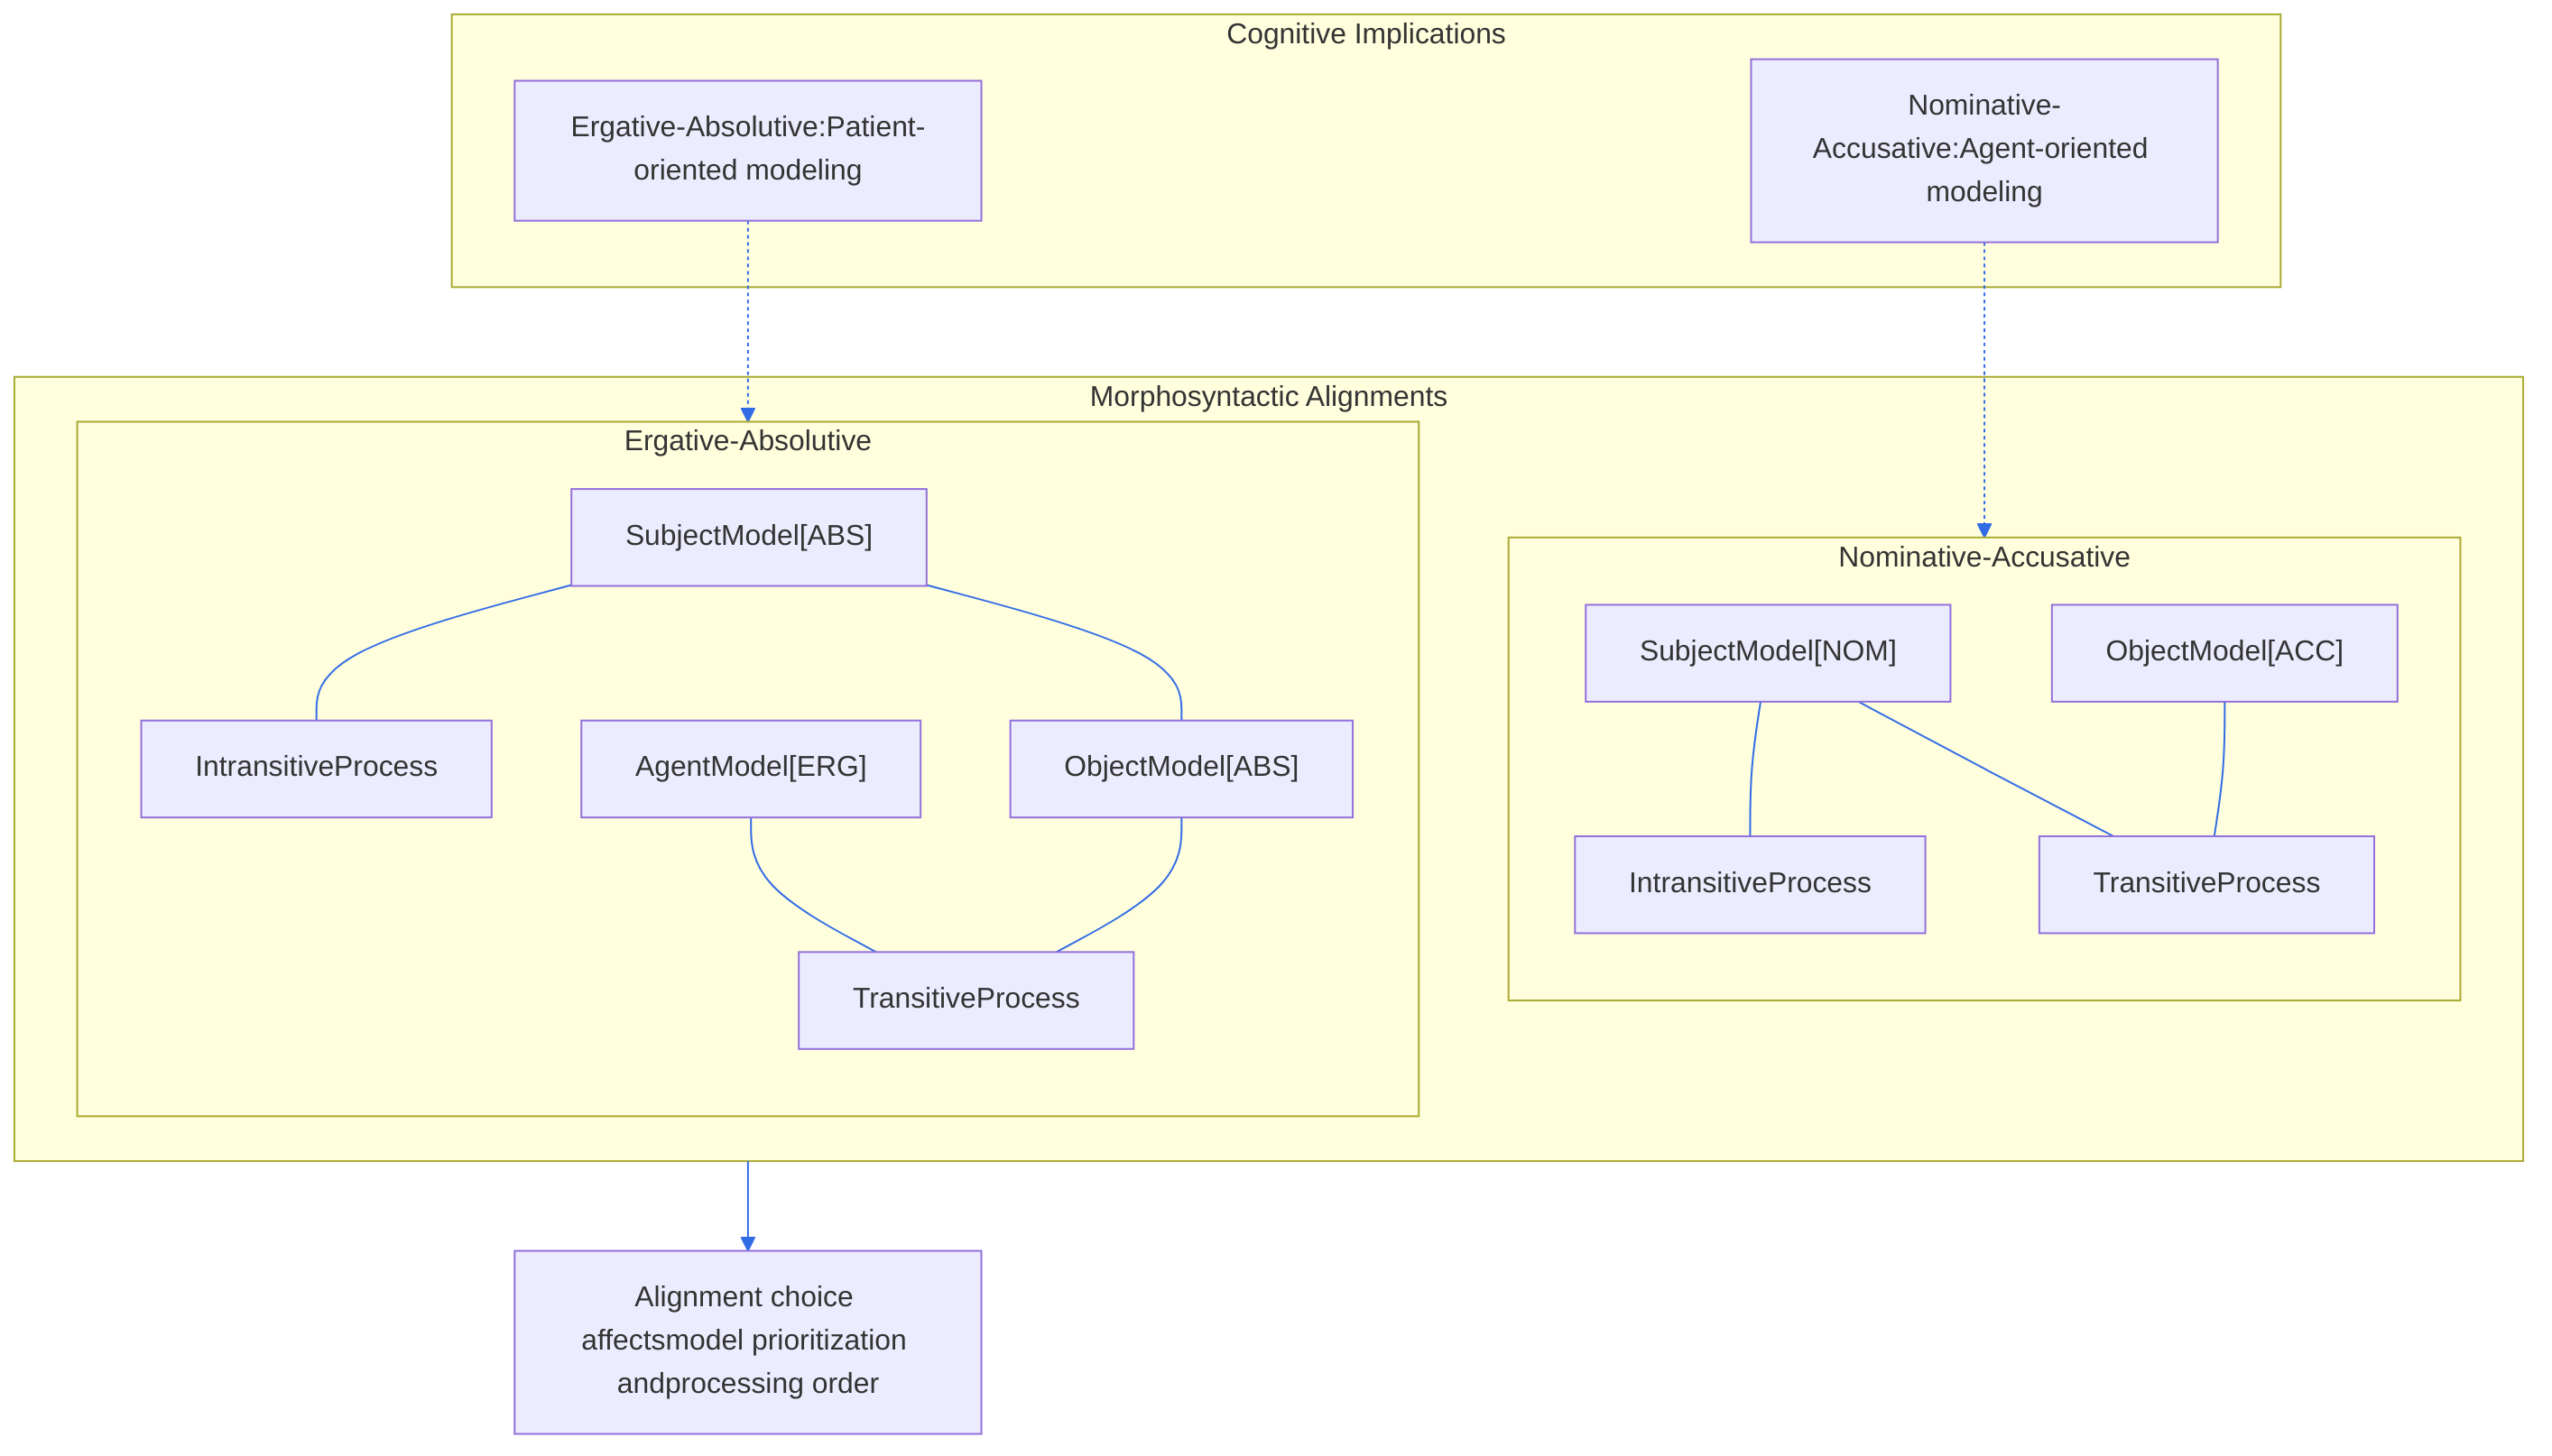
\includegraphics{output/Figure_9.png}
\caption{Morphosyntactic Alignments in Model Relationships. Shows how
CEREBRUM implements different alignment patterns for model relationships
based on linguistic morphosyntactic structures.}
\end{figure}

Figure 10 demonstrates the practical implementation of these alignment
patterns in model ecosystems, showing how different alignment systems
affect model interactions and transformations. The diagram illustrates
the computational implications of each alignment pattern, including
resource allocation, message passing, and transformation efficiency.
This implementation view complements the theoretical alignment patterns
shown in Figure 9 by demonstrating their practical application in
cognitive model management.

\begin{figure}
\centering
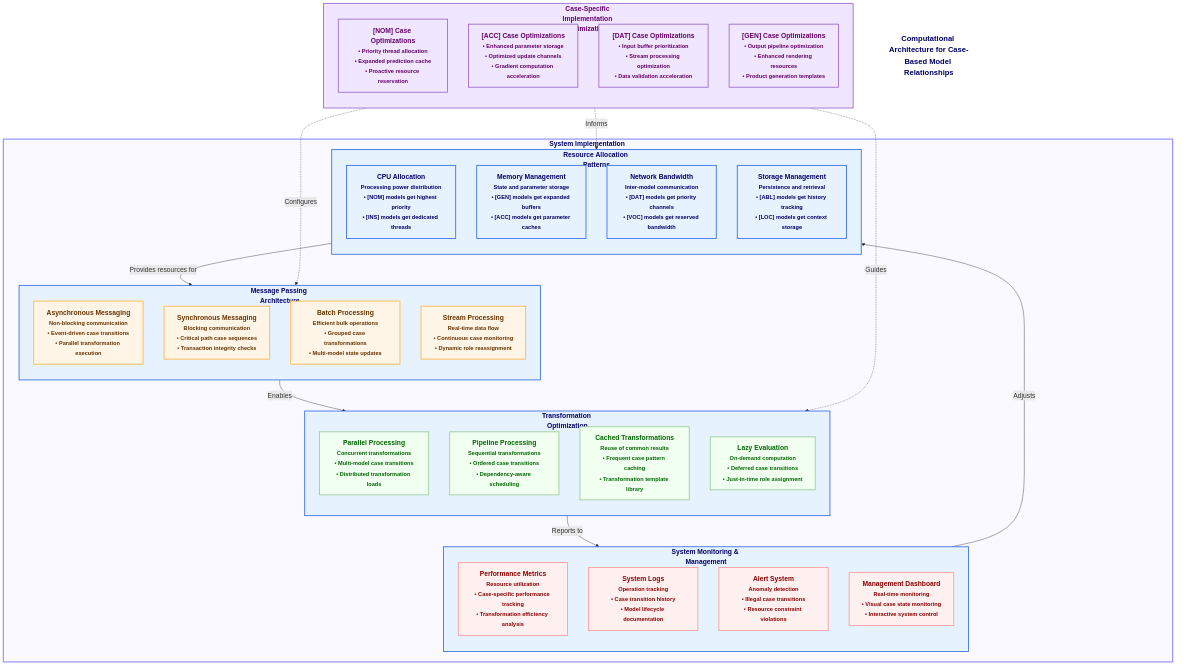
\includegraphics{output/Figure_10.png}
\caption{Computational Implementation of Model Relationships.
Illustrates the practical implementation details of model relationships
in CEREBRUM, including resource allocation patterns, message passing
efficiency, and transformation optimization strategies.}
\end{figure}

\hypertarget{implementation-in-intelligence-production}{%
\section{Implementation in Intelligence
Production}\label{implementation-in-intelligence-production}}

As mentioned, CEREBRUM integrates with intelligence case management
through structured workflows (see Figures 4 and 6). Figure 11 and Figure
12 provide alternative state-based visualizations of these workflows.

\begin{figure}
\centering
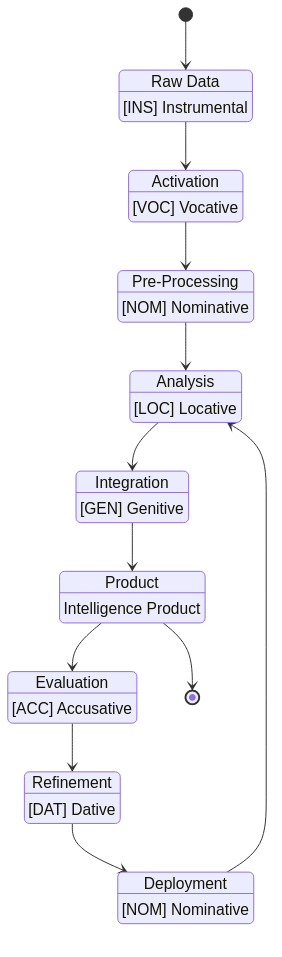
\includegraphics{output/Figure_11.png}
\caption{Implementation in Intelligence Production - State Diagram.
Provides a state-based view of the intelligence workflow highlighting
model case assignments at each stage.}
\end{figure}

\begin{figure}
\centering
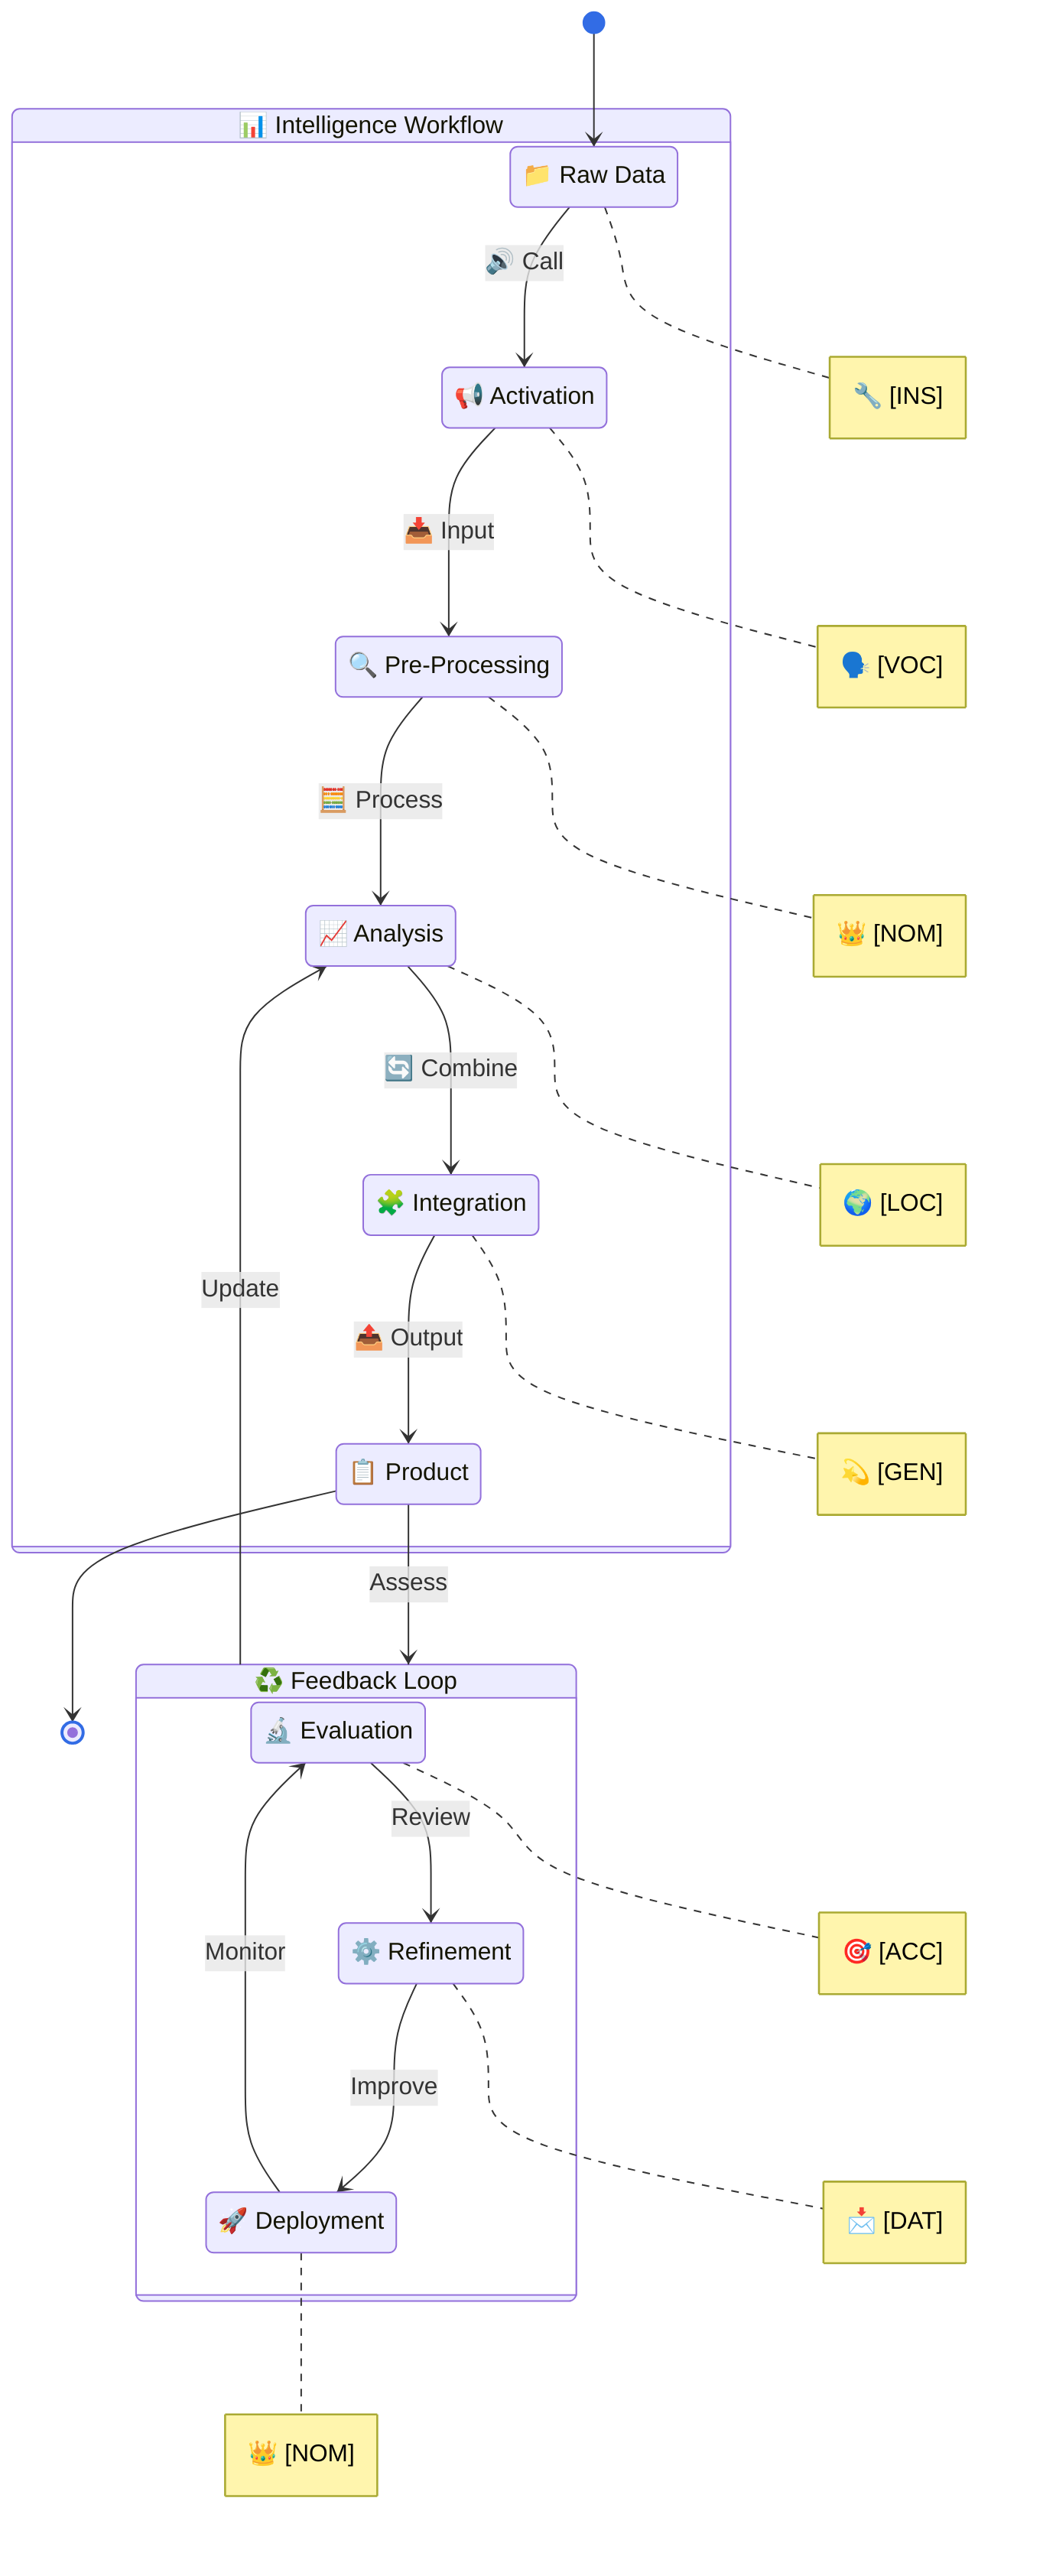
\includegraphics{output/Figure_12.png}
\caption{Intelligence Workflow (Alternative View). Presents another
perspective on the intelligence production cycle and feedback loops,
emphasizing case roles.}
\end{figure}

The intelligence production workflow begins with raw data collection,
where models in instrumental case {[}INS{]} serve as data collection
tools, implementing specific methods for information gathering. As data
moves through preprocessing, models transition to nominative case
{[}NOM{]}, taking on active processing roles to clean, normalize, and
prepare the data for analysis. During analysis, models assume locative
case {[}LOC{]}, providing contextual understanding and environmental
parameters that shape the analytical process.

Integration represents a critical transition point where models in
genitive case {[}GEN{]} generate intelligence products by synthesizing
information from multiple sources. These products then undergo
evaluation by models in accusative case {[}ACC{]}, which assess quality
and identify areas for improvement. The refinement phase employs models
in dative case {[}DAT{]} to process feedback and implement necessary
changes, while deployment returns models to nominative case {[}NOM{]}
for active implementation of refined solutions.

This cyclical process demonstrates how case transformations enable
models to maintain their core identity while adapting to different
functional requirements throughout the intelligence production
lifecycle. Each case assignment optimizes specific aspects of model
behavior, from data collection and processing to product generation and
quality assessment, creating a flexible yet structured approach to
intelligence production.

\hypertarget{active-inference-integration}{%
\section{Active Inference
Integration}\label{active-inference-integration}}

CEREBRUM aligns with active inference frameworks by treating case
transformations as predictive processes within a free energy
minimization framework, as illustrated in Figure 13. Figure 14 details
the associated message passing rules.

\begin{figure}
\centering
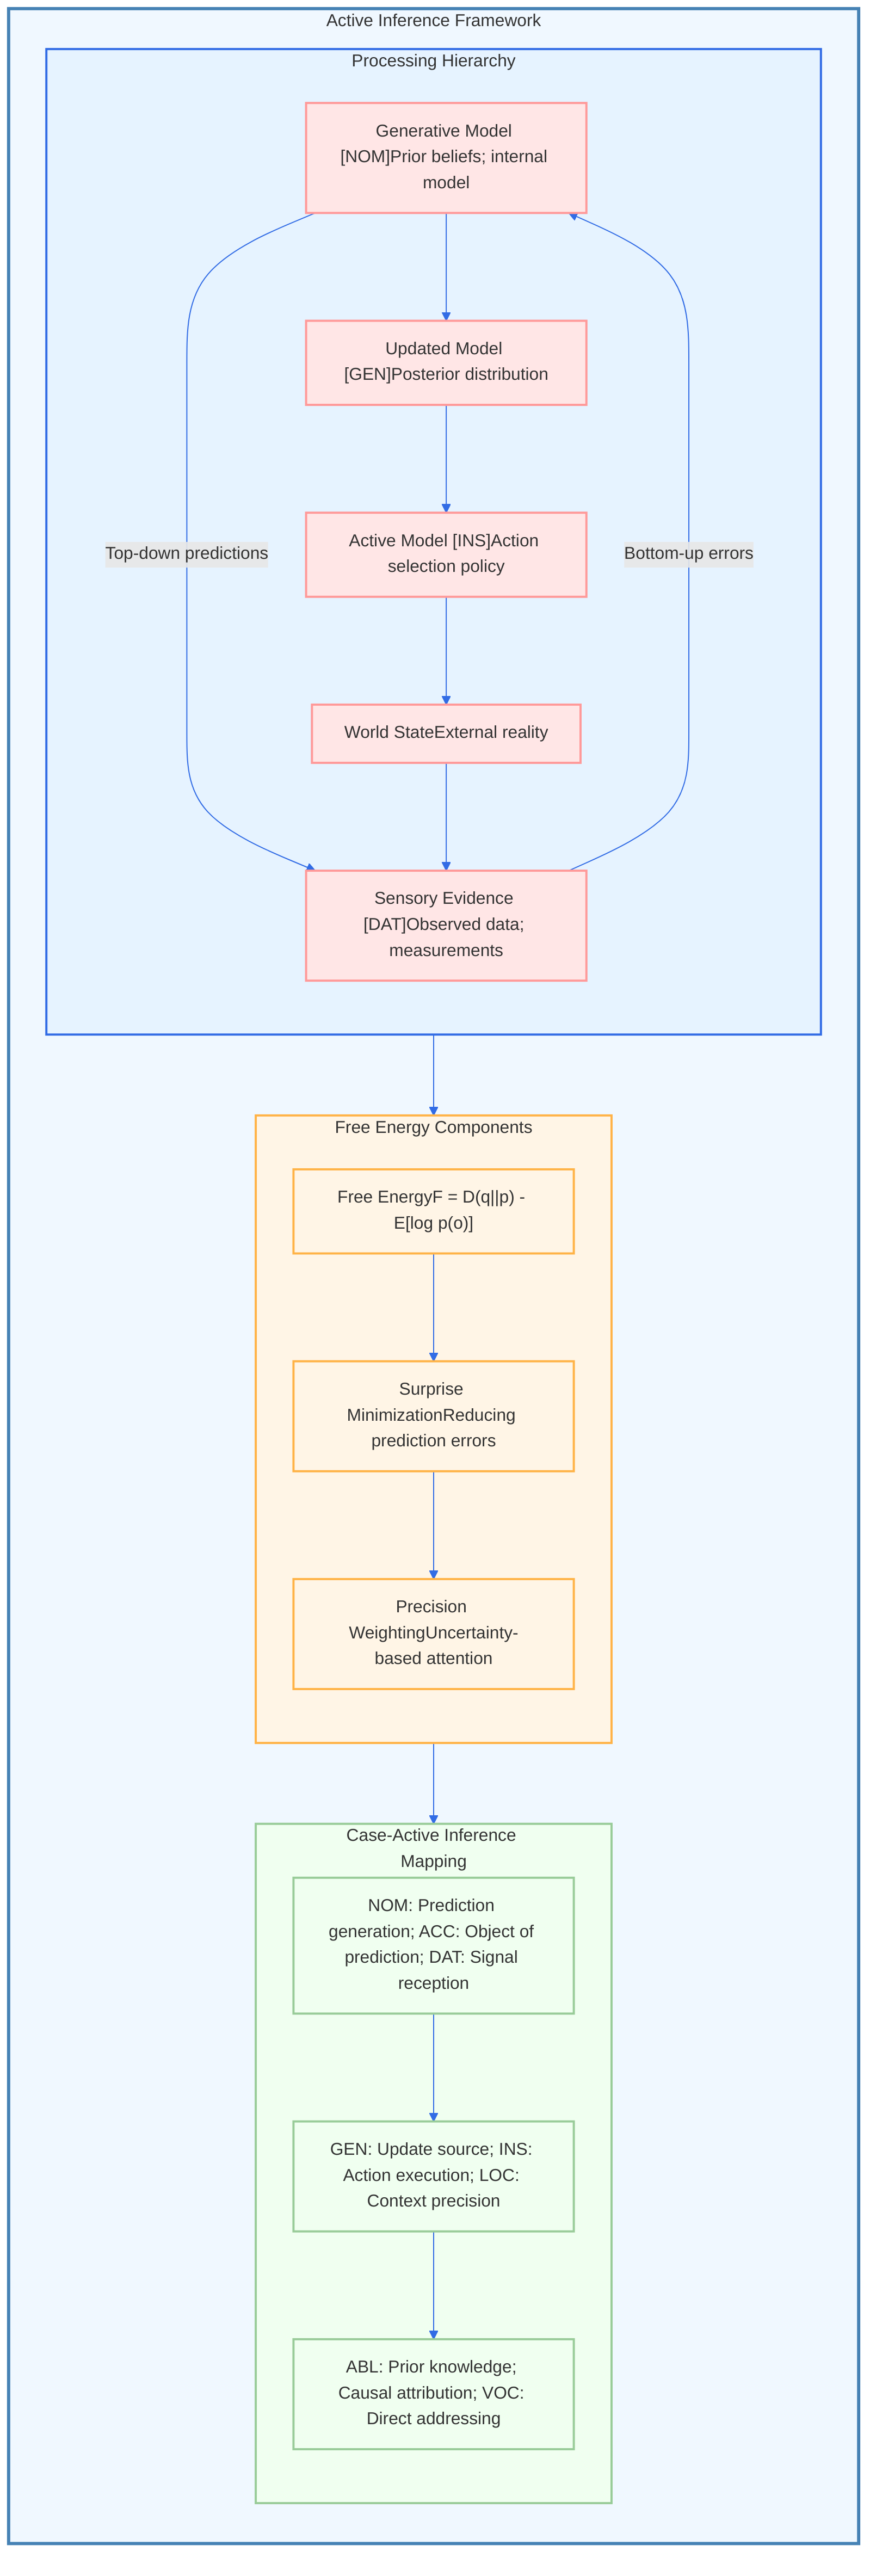
\includegraphics{output/Figure_13.png}
\caption{Active Inference Integration Framework. Shows how active
inference principles are integrated with case transformations through
precision-weighted message passing and free energy minimization.}
\end{figure}

\begin{figure}
\centering
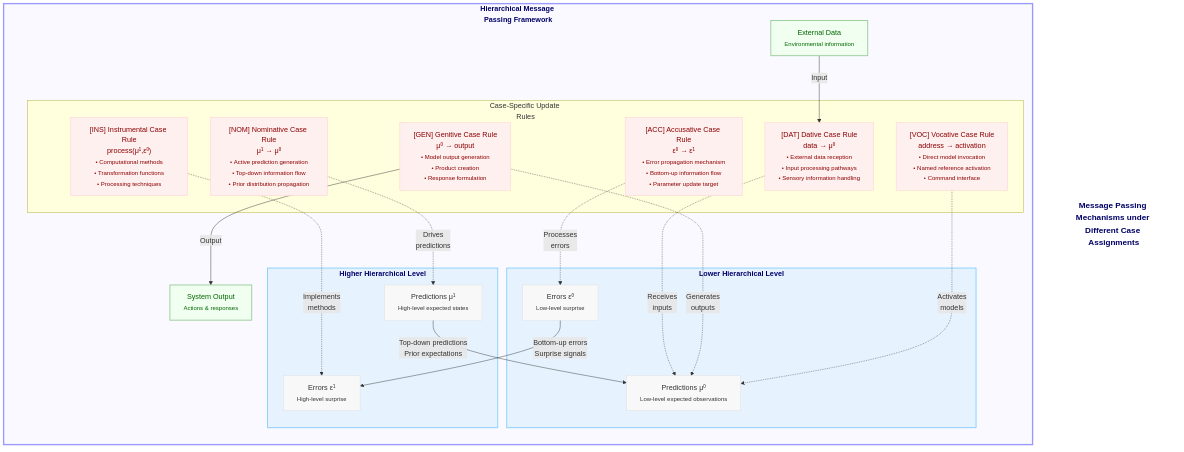
\includegraphics{output/Figure_14.png}
\caption{Case-Specific Message Passing in Active Inference. Illustrates
how message passing dynamics change based on the model's current case
assignment within an active inference hierarchy.}
\end{figure}

\hypertarget{formal-case-calculus}{%
\section{Formal Case Calculus}\label{formal-case-calculus}}

The relationships between case-bearing models follow a formal calculus
derived from grammatical case systems, presented in Figure 15.

\begin{figure}
\centering
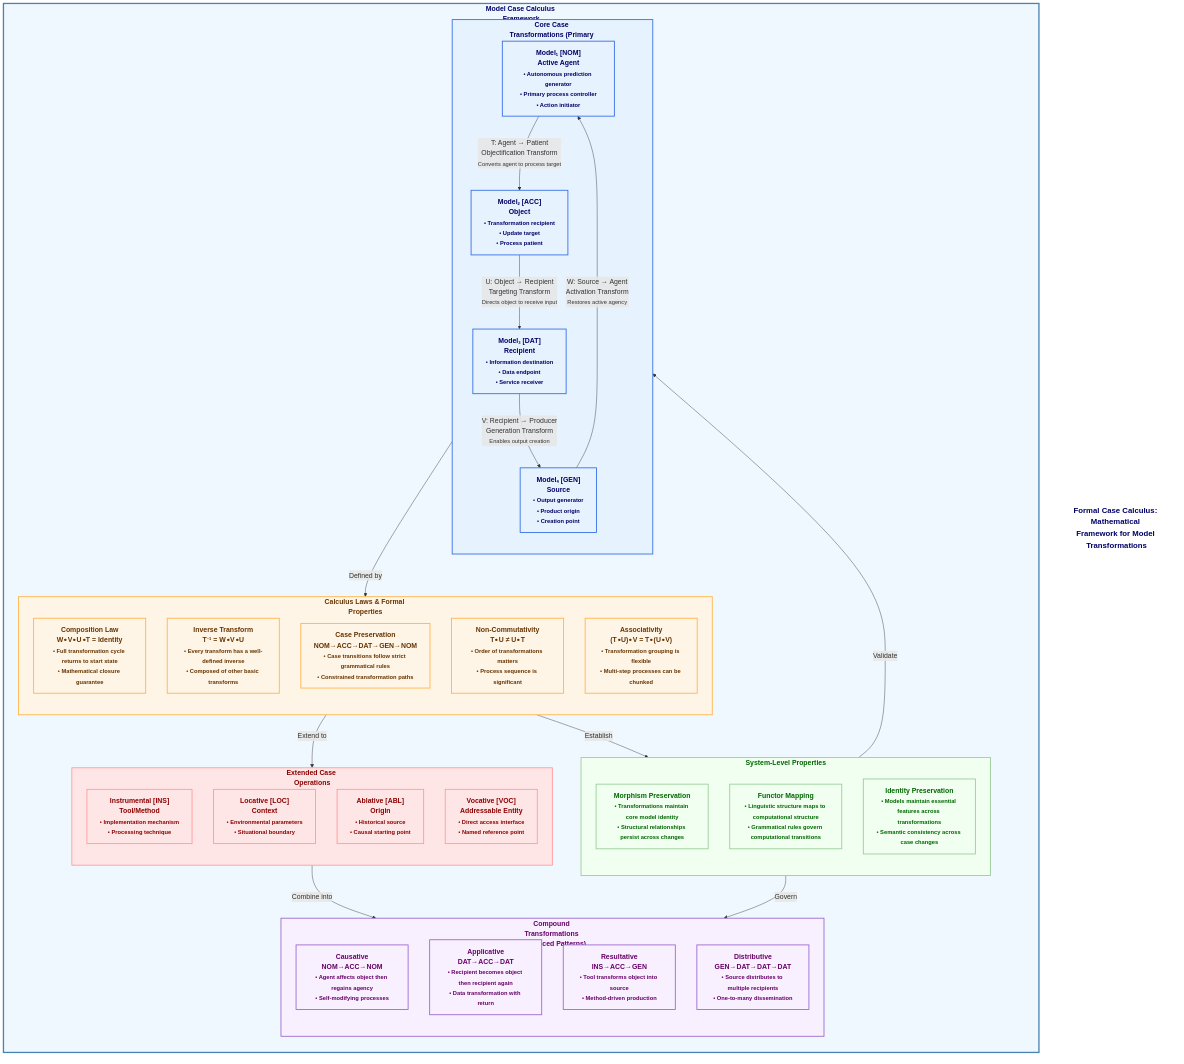
\includegraphics{output/Figure_15.png}
\caption{Model Case Calculus Framework. Presents the formal mathematical
relationships and transformation rules that govern case transitions in
the CEREBRUM framework.}
\end{figure}

\hypertarget{cross-domain-integration-benefits}{%
\section{Cross-Domain Integration
Benefits}\label{cross-domain-integration-benefits}}

The CEREBRUM framework delivers several advantages through its
integration of the four foundational domains:

\textbf{Table 4: Cross-Domain Integration Benefits in CEREBRUM
Framework}

\begin{longtable}[]{@{}llll@{}}
\toprule
\begin{minipage}[b]{0.10\columnwidth}\raggedright
Domain\strut
\end{minipage} & \begin{minipage}[b]{0.18\columnwidth}\raggedright
Contribution\strut
\end{minipage} & \begin{minipage}[b]{0.27\columnwidth}\raggedright
Benefit to CEREBRUM\strut
\end{minipage} & \begin{minipage}[b]{0.33\columnwidth}\raggedright
Theoretical Significance\strut
\end{minipage}\tabularnewline
\midrule
\endhead
\begin{minipage}[t]{0.10\columnwidth}\raggedright
\textbf{Linguistic Case Systems}\strut
\end{minipage} & \begin{minipage}[t]{0.18\columnwidth}\raggedright
Systematic relationship framework; grammatical role templates;
morphosyntactic structures\strut
\end{minipage} & \begin{minipage}[t]{0.27\columnwidth}\raggedright
Structured representation of model interactions; formalized functional
transitions; systematic role assignment\strut
\end{minipage} & \begin{minipage}[t]{0.33\columnwidth}\raggedright
Provides formal semantics for model relationships; enables compositional
theory of model interactions; grounds functions in linguistic
universals\strut
\end{minipage}\tabularnewline
\begin{minipage}[t]{0.10\columnwidth}\raggedright
\textbf{Cognitive Systems Modeling}\strut
\end{minipage} & \begin{minipage}[t]{0.18\columnwidth}\raggedright
Entity representation and processing; model formalization;
information-processing structures\strut
\end{minipage} & \begin{minipage}[t]{0.27\columnwidth}\raggedright
Flexible model instantiation across functional roles; adaptive model
morphology; unified modeling paradigm\strut
\end{minipage} & \begin{minipage}[t]{0.33\columnwidth}\raggedright
Advances theory of cognitive model composition; formalizes functional
transitions in cognitive systems; bridges symbolic and statistical
approaches\strut
\end{minipage}\tabularnewline
\begin{minipage}[t]{0.10\columnwidth}\raggedright
\textbf{Active Inference}\strut
\end{minipage} & \begin{minipage}[t]{0.18\columnwidth}\raggedright
Predictive transformation mechanics; free energy principles;
precision-weighted learning\strut
\end{minipage} & \begin{minipage}[t]{0.27\columnwidth}\raggedright
Self-optimizing workflows with error minimization; principled
uncertainty handling; bidirectional message passing\strut
\end{minipage} & \begin{minipage}[t]{0.33\columnwidth}\raggedright
Extends active inference to model ecosystems; provides mathematical
foundation for case transformations; unifies perception and model
management\strut
\end{minipage}\tabularnewline
\begin{minipage}[t]{0.10\columnwidth}\raggedright
\textbf{Intelligence Production}\strut
\end{minipage} & \begin{minipage}[t]{0.18\columnwidth}\raggedright
Practical operational context; analytical workflows; intelligence cycle
formalisms\strut
\end{minipage} & \begin{minipage}[t]{0.27\columnwidth}\raggedright
Real-world application in case management systems; operational
coherence; analytical integrity\strut
\end{minipage} & \begin{minipage}[t]{0.33\columnwidth}\raggedright
Bridges theoretical and applied intelligence; enhances intelligence
workflow coherence; improves analytical product quality\strut
\end{minipage}\tabularnewline
\bottomrule
\end{longtable}

\hypertarget{related-work}{%
\section{Related Work}\label{related-work}}

CEREBRUM builds upon several research traditions while offering a novel
synthesis. In this first paper, there are no specific works linked or
cited. Later work will provide more detail in reference and derivation.
The work stands transparently on the shoulders of nestmates and so is
presented initially as a speculative design checkpoint in the
development of certain cognitive modeling practices.

Related approaches include:

\hypertarget{cognitive-architectures}{%
\subsection{Cognitive Architectures}\label{cognitive-architectures}}

Existing cognitive architectures such as ACT-R, Soar, and CLARION
provide comprehensive frameworks for modeling cognitive processes but
lack formal mechanisms for representing functional role transitions.
Unlike these systems, CEREBRUM explicitly models the morphological
transformations of computational entities as they move through different
processing contexts.

\hypertarget{category-theoretic-cognition}{%
\subsection{Category-Theoretic
Cognition}\label{category-theoretic-cognition}}

Recent work applying category theory to cognitive science has
established mathematical foundations for cognitive processes. CEREBRUM
extends this tradition by applying categorical structures specifically
to case relationships and active inference, focusing on practical
applications in intelligence production rather than purely theoretical
constructs.

\hypertarget{active-inference-applications}{%
\subsection{Active Inference
Applications}\label{active-inference-applications}}

Prior applications of active inference to artificial intelligence have
focused primarily on perception and action in individual agents.
CEREBRUM expands this domain by applying active inference principles to
model ecosystems, where multiple models interact within structured
workflows guided by case-based transformations.

\hypertarget{linguistic-computing}{%
\subsection{Linguistic Computing}\label{linguistic-computing}}

Computational linguistics has extensively employed case grammar for
natural language processing, but rarely extended these principles to
model management. CEREBRUM repurposes linguistic case theory as a
structural framework for model relationships rather than textual
analysis.

\hypertarget{practical-applications-of-model-declension-in-cognitive-ecosystems}{%
\section{Practical Applications of Model Declension in Cognitive
Ecosystems}\label{practical-applications-of-model-declension-in-cognitive-ecosystems}}

The declension paradigm for cognitive models offers practical benefits
in complex model ecosystems spanning multiple cognitive domains. This
section outlines specific applications where the morphological
adaptability of models provides significant advantages.

\hypertarget{model-pipeline-optimization}{%
\subsection{Model Pipeline
Optimization}\label{model-pipeline-optimization}}

Complex cognitive workflows typically involve sequences of models
arranged in processing pipelines. Traditional approaches require
specialized interface layers between models, leading to inefficiencies
and compatibility challenges. By applying case declensions to models in
these pipelines, each component can seamlessly adapt its interfaces:

Consider a pipeline where Model₂ exhibits a case transition from
{[}ACC{]} (receiving data) to {[}DAT{]} (forwarding results),
demonstrating how a single model can adapt its functional interfaces
based on its position in the processing sequence.

\hypertarget{computational-resource-optimization}{%
\subsection{Computational Resource
Optimization}\label{computational-resource-optimization}}

In resource-constrained environments, the precision allocation mechanism
provided by case declension enables dynamic distribution of
computational resources:

\textbf{Table 5: Resource Allocation Strategy by Cognitive Task Type}

\begin{longtable}[]{@{}llll@{}}
\toprule
\begin{minipage}[b]{0.13\columnwidth}\raggedright
Use Case\strut
\end{minipage} & \begin{minipage}[b]{0.24\columnwidth}\raggedright
Resource Strategy\strut
\end{minipage} & \begin{minipage}[b]{0.19\columnwidth}\raggedright
Case Priority\strut
\end{minipage} & \begin{minipage}[b]{0.32\columnwidth}\raggedright
Optimization Objective\strut
\end{minipage}\tabularnewline
\midrule
\endhead
\begin{minipage}[t]{0.13\columnwidth}\raggedright
Real-time decision making\strut
\end{minipage} & \begin{minipage}[t]{0.24\columnwidth}\raggedright
Prioritize prediction generation; allocate resources to forward
inference; minimize predictive latency\strut
\end{minipage} & \begin{minipage}[t]{0.19\columnwidth}\raggedright
{[}NOM{]} \textgreater{} {[}DAT{]} \textgreater{} {[}ACC{]}
\textgreater{} others\strut
\end{minipage} & \begin{minipage}[t]{0.32\columnwidth}\raggedright
Minimize latency; maximize predictive accuracy; optimize decision
boundaries\strut
\end{minipage}\tabularnewline
\begin{minipage}[t]{0.13\columnwidth}\raggedright
Data ingestion and processing\strut
\end{minipage} & \begin{minipage}[t]{0.24\columnwidth}\raggedright
Prioritize input handling; allocate resources to perceptual
categorization; maximize throughput\strut
\end{minipage} & \begin{minipage}[t]{0.19\columnwidth}\raggedright
{[}DAT{]} \textgreater{} {[}ACC{]} \textgreater{} {[}GEN{]}
\textgreater{} others\strut
\end{minipage} & \begin{minipage}[t]{0.32\columnwidth}\raggedright
Maximize throughput; optimize filter efficiency; minimize information
loss\strut
\end{minipage}\tabularnewline
\begin{minipage}[t]{0.13\columnwidth}\raggedright
Report generation\strut
\end{minipage} & \begin{minipage}[t]{0.24\columnwidth}\raggedright
Prioritize output production; allocate resources to synthesis; optimize
presentation clarity\strut
\end{minipage} & \begin{minipage}[t]{0.19\columnwidth}\raggedright
{[}GEN{]} \textgreater{} {[}NOM{]} \textgreater{} {[}LOC{]}
\textgreater{} others\strut
\end{minipage} & \begin{minipage}[t]{0.32\columnwidth}\raggedright
Optimize fidelity; maximize clarity; ensure appropriate detail
level\strut
\end{minipage}\tabularnewline
\begin{minipage}[t]{0.13\columnwidth}\raggedright
Method development\strut
\end{minipage} & \begin{minipage}[t]{0.24\columnwidth}\raggedright
Prioritize process refinement; allocate resources to algorithm
optimization; focus on error reduction\strut
\end{minipage} & \begin{minipage}[t]{0.19\columnwidth}\raggedright
{[}INS{]} \textgreater{} {[}ACC{]} \textgreater{} {[}NOM{]}
\textgreater{} others\strut
\end{minipage} & \begin{minipage}[t]{0.32\columnwidth}\raggedright
Minimize error; improve algorithmic efficiency; enhance procedural
robustness\strut
\end{minipage}\tabularnewline
\bottomrule
\end{longtable}

This dynamic resource allocation is formalized through the
precision-weighted free energy equation (Equation 14 in the Mathematical
Appendix), where models are allocated computational resources
proportional to their precision weights for their current case
assignment.

\hypertarget{model-ecosystem-adaptability}{%
\subsection{Model Ecosystem
Adaptability}\label{model-ecosystem-adaptability}}

Cognitive ecosystems must adapt to changing environments and
requirements. The declension paradigm enables flexible reconfiguration
of model relationships without architectural redesign.

Conceptually, this means the same set of models can reconfigure their
functional roles through case reassignment, adapting to new requirements
without changing the underlying model implementations.

\hypertarget{cross-domain-integration}{%
\subsection{Cross-Domain Integration}\label{cross-domain-integration}}

The CEREBRUM framework facilitates integration between disparate
cognitive domains by providing a unified grammatical structure for model
interactions:

\textbf{Table 6: Cross-Domain Integration Patterns in CEREBRUM
Framework}

\begin{longtable}[]{@{}llll@{}}
\toprule
\begin{minipage}[b]{0.11\columnwidth}\raggedright
Domain\strut
\end{minipage} & \begin{minipage}[b]{0.20\columnwidth}\raggedright
Primary Cases\strut
\end{minipage} & \begin{minipage}[b]{0.30\columnwidth}\raggedright
Integration Pattern\strut
\end{minipage} & \begin{minipage}[b]{0.27\columnwidth}\raggedright
Error Propagation\strut
\end{minipage}\tabularnewline
\midrule
\endhead
\begin{minipage}[t]{0.11\columnwidth}\raggedright
\textbf{Perception}\strut
\end{minipage} & \begin{minipage}[t]{0.20\columnwidth}\raggedright
{[}NOM{]} (senses), {[}ACC{]} (percepts)\strut
\end{minipage} & \begin{minipage}[t]{0.30\columnwidth}\raggedright
Sensory models {[}NOM{]} → Perceptual models {[}ACC{]}; hierarchical
feature extraction; predictive sensing\strut
\end{minipage} & \begin{minipage}[t]{0.27\columnwidth}\raggedright
Bottom-up; prediction errors flow from sensors to percepts;
precision-weighted by sensory reliability\strut
\end{minipage}\tabularnewline
\begin{minipage}[t]{0.11\columnwidth}\raggedright
\textbf{Reasoning}\strut
\end{minipage} & \begin{minipage}[t]{0.20\columnwidth}\raggedright
{[}INS{]} (logic), {[}LOC{]} (context)\strut
\end{minipage} & \begin{minipage}[t]{0.30\columnwidth}\raggedright
Logical models {[}INS{]} → Contextual models {[}LOC{]};
context-sensitive inference; situational logic\strut
\end{minipage} & \begin{minipage}[t]{0.27\columnwidth}\raggedright
Bidirectional; coherence errors propagate between logical rules and
contextual constraints; mutual constraints\strut
\end{minipage}\tabularnewline
\begin{minipage}[t]{0.11\columnwidth}\raggedright
\textbf{Planning}\strut
\end{minipage} & \begin{minipage}[t]{0.20\columnwidth}\raggedright
{[}GEN{]} (goals), {[}ABL{]} (history)\strut
\end{minipage} & \begin{minipage}[t]{0.30\columnwidth}\raggedright
Historical models {[}ABL{]} → Goal models {[}GEN{]}; experience-informed
planning; trajectory optimization\strut
\end{minipage} & \begin{minipage}[t]{0.27\columnwidth}\raggedright
Top-down; goal-directed errors influence historical interpretation;
teleological constraints\strut
\end{minipage}\tabularnewline
\begin{minipage}[t]{0.11\columnwidth}\raggedright
\textbf{Action}\strut
\end{minipage} & \begin{minipage}[t]{0.20\columnwidth}\raggedright
{[}DAT{]} (commands), {[}NOM{]} (execution)\strut
\end{minipage} & \begin{minipage}[t]{0.30\columnwidth}\raggedright
Command models {[}DAT{]} → Execution models {[}NOM{]}; imperative
processing; motor control\strut
\end{minipage} & \begin{minipage}[t]{0.27\columnwidth}\raggedright
Circular; execution errors feed back to command refinement; continuous
adjustment loop\strut
\end{minipage}\tabularnewline
\bottomrule
\end{longtable}

By mapping these domain-specific interactions to standardized case
relationships, previously incompatible models can be integrated into
cohesive cognitive systems.

\hypertarget{knowledge-graph-enhancement}{%
\subsection{Knowledge Graph
Enhancement}\label{knowledge-graph-enhancement}}

The case declension system enhances knowledge representation by
providing richer relational semantics in model-based knowledge graphs.
This enhancement operates at multiple levels:

\begin{enumerate}
\def\labelenumi{\arabic{enumi}.}
\tightlist
\item
  \textbf{Semantic Role Labeling}:

  \begin{itemize}
  \tightlist
  \item
    Models in {[}NOM{]} case represent active knowledge producers
  \item
    Models in {[}ACC{]} case represent knowledge targets/recipients
  \item
    Models in {[}DAT{]} case represent knowledge transfer endpoints
  \item
    Models in {[}GEN{]} case represent knowledge sources/origins
  \item
    Models in {[}INS{]} case represent methodological knowledge
  \item
    Models in {[}LOC{]} case represent contextual knowledge
  \item
    Models in {[}ABL{]} case represent historical/causal knowledge
  \end{itemize}
\item
  \textbf{Relationship Typing}:

  \begin{itemize}
  \tightlist
  \item
    Morphosyntactic edges encode relationship types
  \item
    Case assignments provide edge directionality
  \item
    Case transitions represent knowledge flow patterns
  \item
    Multi-case paths represent complex knowledge transformations
  \end{itemize}
\item
  \textbf{Example Knowledge Propagation Rules}:

  \begin{itemize}
  \tightlist
  \item
    Case-preserving transformations maintain semantic roles
  \item
    Case-changing transformations represent functional shifts
  \item
    Case alignment patterns guide knowledge integration
  \item
    Case-based precision weighting prioritizes knowledge flow (see
    Equation 13 in Mathematical Appendix)
  \end{itemize}
\end{enumerate}

This enhanced knowledge graph shows how case-declined models provide
explicit relationship semantics between entities, creating richer
knowledge representations that mirror the way natural language encodes
semantic relationships through case systems.

\hypertarget{emergent-behaviors-in-model-collectives}{%
\subsection{Emergent Behaviors in Model
Collectives}\label{emergent-behaviors-in-model-collectives}}

When multiple case-bearing models interact within an ecosystem, emergent
collective behaviors arise from their case-driven interactions,
analogous to how linguistic communities develop shared understanding
through dialog:

\begin{enumerate}
\def\labelenumi{\arabic{enumi}.}
\tightlist
\item
  \textbf{Self-organizing workflows}:

  \begin{itemize}
  \tightlist
  \item
    Models dynamically form processing chains based on complementary
    case assignments
  \item
    Like speakers in dialogue naturally assuming complementary roles
    (questioner/answerer)
  \item
    Case alignment creates natural processing pipelines
  \item
    Processing chains form spontaneously through case compatibility
  \end{itemize}
\item
  \textbf{Adaptive resource allocation}:

  \begin{itemize}
  \tightlist
  \item
    Precision-weighted competition for computational resources drives
    efficient task distribution
  \item
    Similar to attention allocation in linguistic communities
  \item
    Resources are allocated based on case-specific precision weights
    (see Equation 13 in the Mathematical Appendix)
  \item
    Dynamic reallocation follows free energy gradients
  \end{itemize}
\item
  \textbf{Collective learning}:

  \begin{itemize}
  \tightlist
  \item
    Error signals propagate through case relationships
  \item
    Like linguistic communities converging on shared meanings
  \item
    Learning rates are modulated by case compatibility
  \item
    System-wide adaptation through message passing (see Equations 8-12
    in the Mathematical Appendix)
  \end{itemize}
\item
  \textbf{Fault tolerance}:

  \begin{itemize}
  \tightlist
  \item
    Models can adopt alternative cases when certain cognitive functions
    are degraded
  \item
    Similar to linguistic communities adapting to speaker limitations
  \item
    Case reassignment follows free energy minimization
  \item
    Graceful degradation through case flexibility
  \end{itemize}
\item
  \textbf{Semantic Consensus Formation}:

  \begin{itemize}
  \tightlist
  \item
    Models converge on shared representations through case-mediated
    interactions
  \item
    Parallels linguistic communities developing shared vocabularies
  \item
    Consensus emerges through case-specific alignment
  \item
    Alignment strength varies by case type
  \end{itemize}
\item
  \textbf{Hierarchical Organization}:

  \begin{itemize}
  \tightlist
  \item
    Case relationships naturally create processing hierarchies
  \item
    Like linguistic communities developing formal/informal speech levels
  \item
    Hierarchy levels emerge from case distributions
  \item
    Case assignments reflect hierarchical position
  \end{itemize}
\end{enumerate}

These emergent properties demonstrate how the declension paradigm
enables robust, adaptive collective behaviors in complex cognitive
ecosystems, mirroring the way linguistic communities develop and
maintain shared understanding through structured interactions. The
mathematical formalization of these properties provides a rigorous
foundation for analyzing and optimizing model collective behavior.

The parallel between model collectives and linguistic communities
extends to:

\begin{enumerate}
\def\labelenumi{\arabic{enumi}.}
\tightlist
\item
  \textbf{Information Flow Patterns}:

  \begin{itemize}
  \tightlist
  \item
    Case-based routing: Messages flow according to case compatibility
  \item
    Community structure: Models cluster by case affinity
  \item
    Flow efficiency depends on case-specific precision weights
  \end{itemize}
\item
  \textbf{Adaptation Mechanisms}:

  \begin{itemize}
  \tightlist
  \item
    Local adjustments: Models modify case assignments based on neighbors
  \item
    Global optimization: System-wide free energy minimization (see
    Equation 1 in the Mathematical Appendix)
  \item
    Adaptation rates follow temporal decay patterns
  \end{itemize}
\item
  \textbf{Stability Properties}:

  \begin{itemize}
  \tightlist
  \item
    Case equilibrium: Stable distributions of case assignments
  \item
    Dynamic resilience: Recovery from perturbations
  \item
    Stability emerges from case distribution entropy
  \end{itemize}
\end{enumerate}

This framework provides a formal basis for understanding how collections
of case-bearing models can develop sophisticated collective behaviors
analogous to linguistic communities, while maintaining mathematical
rigor through precise formalization of the underlying mechanisms.

(See Appendix 2: Novel Linguistic Cases for a discussion of how CEREBRUM
can discover and create new linguistic cases beyond traditional case
systems.)

\hypertarget{future-directions}{%
\section{Future Directions}\label{future-directions}}

Future work on the CEREBRUM framework will focus on both theoretical
expansions and practical implementations:

\begin{itemize}
\tightlist
\item
  \textbf{Programming Libraries}: Developing robust programming
  libraries implementing the CEREBRUM framework across multiple
  languages to facilitate adoption
\item
  \textbf{Visualization Tools}: Creating interactive visualization tools
  for case transformation processes to enhance understanding and
  analysis
\item
  \textbf{Linguistic Extensions}: Expanding the framework to incorporate
  additional linguistic features such as aspect, tense, and modality
  into model relationship representations
\item
  \textbf{Open Source Stewardship}: Establishing open source governance
  and community development practices through the Active Inference
  Institute
\item
  \textbf{Computational Complexity}: Deriving formal computational
  complexity estimates for case transformations in various model
  ecosystem configurations
\item
  \textbf{Multiple Dispatch Systems}: Implementing multiple dispatch
  architectures for programming languages to efficiently handle
  case-based polymorphism
\item
  \textbf{Database Methods}: Developing specialized database structures
  and query languages for efficient storage and retrieval of
  case-bearing models
\item
  \textbf{Cognitive Security}: Exploring security implications of
  case-based systems, including authorization frameworks based on case
  relationships
\end{itemize}

\hypertarget{conclusion}{%
\section{Conclusion}\label{conclusion}}

CEREBRUM provides a structured framework for managing cognitive models
by applying linguistic case principles to represent different functional
roles and relationships. This synthesis of linguistic theory, category
mathematics, active inference, and intelligence production creates a
powerful paradigm for understanding and managing complex model
ecosystems. By treating models as case-bearing entities, CEREBRUM
enables more formalized transformations between model states while
providing intuitive metaphors for model relationships that align with
human cognitive patterns and operational intelligence workflows.

The formal integration of variational free energy principles with case
transformations establishes CEREBRUM as a mathematically rigorous
framework for active inference implementations. The precision-weighted
case selection mechanisms, Markov blanket formulations, and hierarchical
message passing structures provide computationally tractable algorithms
for optimizing model interactions. These technical formalizations bridge
theoretical linguistics and practical cognitive modeling while
maintaining mathematical coherence through category-theoretic
validation.

The CEREBRUM framework represents another milestone in a long journey of
how we conceptualize model relationships, moving from ad hoc integration
approaches, on through seeking the first principles of persistent,
composable, linguistic intelligences. This journey, really an adventure,
continues to have profound implications for theory and practice. By here
incipiently formalizing the grammatical structure of model interactions,
CEREBRUM points towards enhancement of current capabilities and opens
new avenues for modeling emergent behaviors in ecosystems of shared
intelligence. As computational systems continue to grow in complexity,
frameworks like CEREBRUM that provide structured yet flexible approaches
to model management will become increasingly essential for maintaining
conceptual coherence and operational effectiveness.

% Here we're inserting a marker to separate where the appendices will be added
% The pandoc command will need to be modified to replace this marker
% with the appendix content and proper ppendix command
__APPENDIX_MARKER__

% After the body content

\end{document}
